\documentclass[1p]{elsarticle_modified}
%\bibliographystyle{elsarticle-num}

%\usepackage[colorlinks]{hyperref}
%\usepackage{abbrmath_seonhwa} %\Abb, \Ascr, \Acal ,\Abf, \Afrak
\usepackage{amsfonts}
\usepackage{amssymb}
\usepackage{amsmath}
\usepackage{amsthm}
\usepackage{scalefnt}
\usepackage{amsbsy}
\usepackage{kotex}
\usepackage{caption}
\usepackage{subfig}
\usepackage{color}
\usepackage{graphicx}
\usepackage{xcolor} %% white, black, red, green, blue, cyan, magenta, yellow
\usepackage{float}
\usepackage{setspace}
\usepackage{hyperref}

\usepackage{tikz}
\usetikzlibrary{arrows}

\usepackage{multirow}
\usepackage{array} % fixed length table
\usepackage{hhline}

%%%%%%%%%%%%%%%%%%%%%
\makeatletter
\renewcommand*\env@matrix[1][\arraystretch]{%
	\edef\arraystretch{#1}%
	\hskip -\arraycolsep
	\let\@ifnextchar\new@ifnextchar
	\array{*\c@MaxMatrixCols c}}
\makeatother %https://tex.stackexchange.com/questions/14071/how-can-i-increase-the-line-spacing-in-a-matrix
%%%%%%%%%%%%%%%

\usepackage[normalem]{ulem}

\newcommand{\msout}[1]{\ifmmode\text{\sout{\ensuremath{#1}}}\else\sout{#1}\fi}
%SOURCE: \msout is \stkout macro in https://tex.stackexchange.com/questions/20609/strikeout-in-math-mode

\newcommand{\cancel}[1]{
	\ifmmode
	{\color{red}\msout{#1}}
	\else
	{\color{red}\sout{#1}}
	\fi
}

\newcommand{\add}[1]{
	{\color{blue}\uwave{#1}}
}

\newcommand{\replace}[2]{
	\ifmmode
	{\color{red}\msout{#1}}{\color{blue}\uwave{#2}}
	\else
	{\color{red}\sout{#1}}{\color{blue}\uwave{#2}}
	\fi
}

\newcommand{\Sol}{\mathcal{S}} %segment
\newcommand{\D}{D} %diagram
\newcommand{\A}{\mathcal{A}} %arc


%%%%%%%%%%%%%%%%%%%%%%%%%%%%%5 test

\def\sl{\operatorname{\textup{SL}}(2,\Cbb)}
\def\psl{\operatorname{\textup{PSL}}(2,\Cbb)}
\def\quan{\mkern 1mu \triangleright \mkern 1mu}

\theoremstyle{definition}
\newtheorem{thm}{Theorem}[section]
\newtheorem{prop}[thm]{Proposition}
\newtheorem{lem}[thm]{Lemma}
\newtheorem{ques}[thm]{Question}
\newtheorem{cor}[thm]{Corollary}
\newtheorem{defn}[thm]{Definition}
\newtheorem{exam}[thm]{Example}
\newtheorem{rmk}[thm]{Remark}
\newtheorem{alg}[thm]{Algorithm}

\newcommand{\I}{\sqrt{-1}}
\begin{document}

%\begin{frontmatter}
%
%\title{Boundary parabolic representations of knots up to 8 crossings}
%
%%% Group authors per affiliation:
%\author{Yunhi Cho} 
%\address{Department of Mathematics, University of Seoul, Seoul, Korea}
%\ead{yhcho@uos.ac.kr}
%
%
%\author{Seonhwa Kim} %\fnref{s_kim}}
%\address{Center for Geometry and Physics, Institute for Basic Science, Pohang, 37673, Korea}
%\ead{ryeona17@ibs.re.kr}
%
%\author{Hyuk Kim}
%\address{Department of Mathematical Sciences, Seoul National University, Seoul 08826, Korea}
%\ead{hyukkim@snu.ac.kr}
%
%\author{Seokbeom Yoon}
%\address{Department of Mathematical Sciences, Seoul National University, Seoul, 08826,  Korea}
%\ead{sbyoon15@snu.ac.kr}
%
%\begin{abstract}
%We find all boundary parabolic representation of knots up to 8 crossings.
%
%\end{abstract}
%\begin{keyword}
%    \MSC[2010] 57M25 
%\end{keyword}
%
%\end{frontmatter}

%\linenumbers
%\tableofcontents
%
\newcommand\colored[1]{\textcolor{white}{\rule[-0.35ex]{0.8em}{1.4ex}}\kern-0.8em\color{red} #1}%
%\newcommand\colored[1]{\textcolor{white}{ #1}\kern-2.17ex	\textcolor{white}{ #1}\kern-1.81ex	\textcolor{white}{ #1}\kern-2.15ex\color{red}#1	}

{\Large $\underline{12a_{0316}~(K12a_{0316})}$}

\setlength{\tabcolsep}{10pt}
\renewcommand{\arraystretch}{1.6}
\vspace{1cm}\begin{tabular}{m{100pt}>{\centering\arraybackslash}m{274pt}}
\multirow{5}{120pt}{
	\centering
	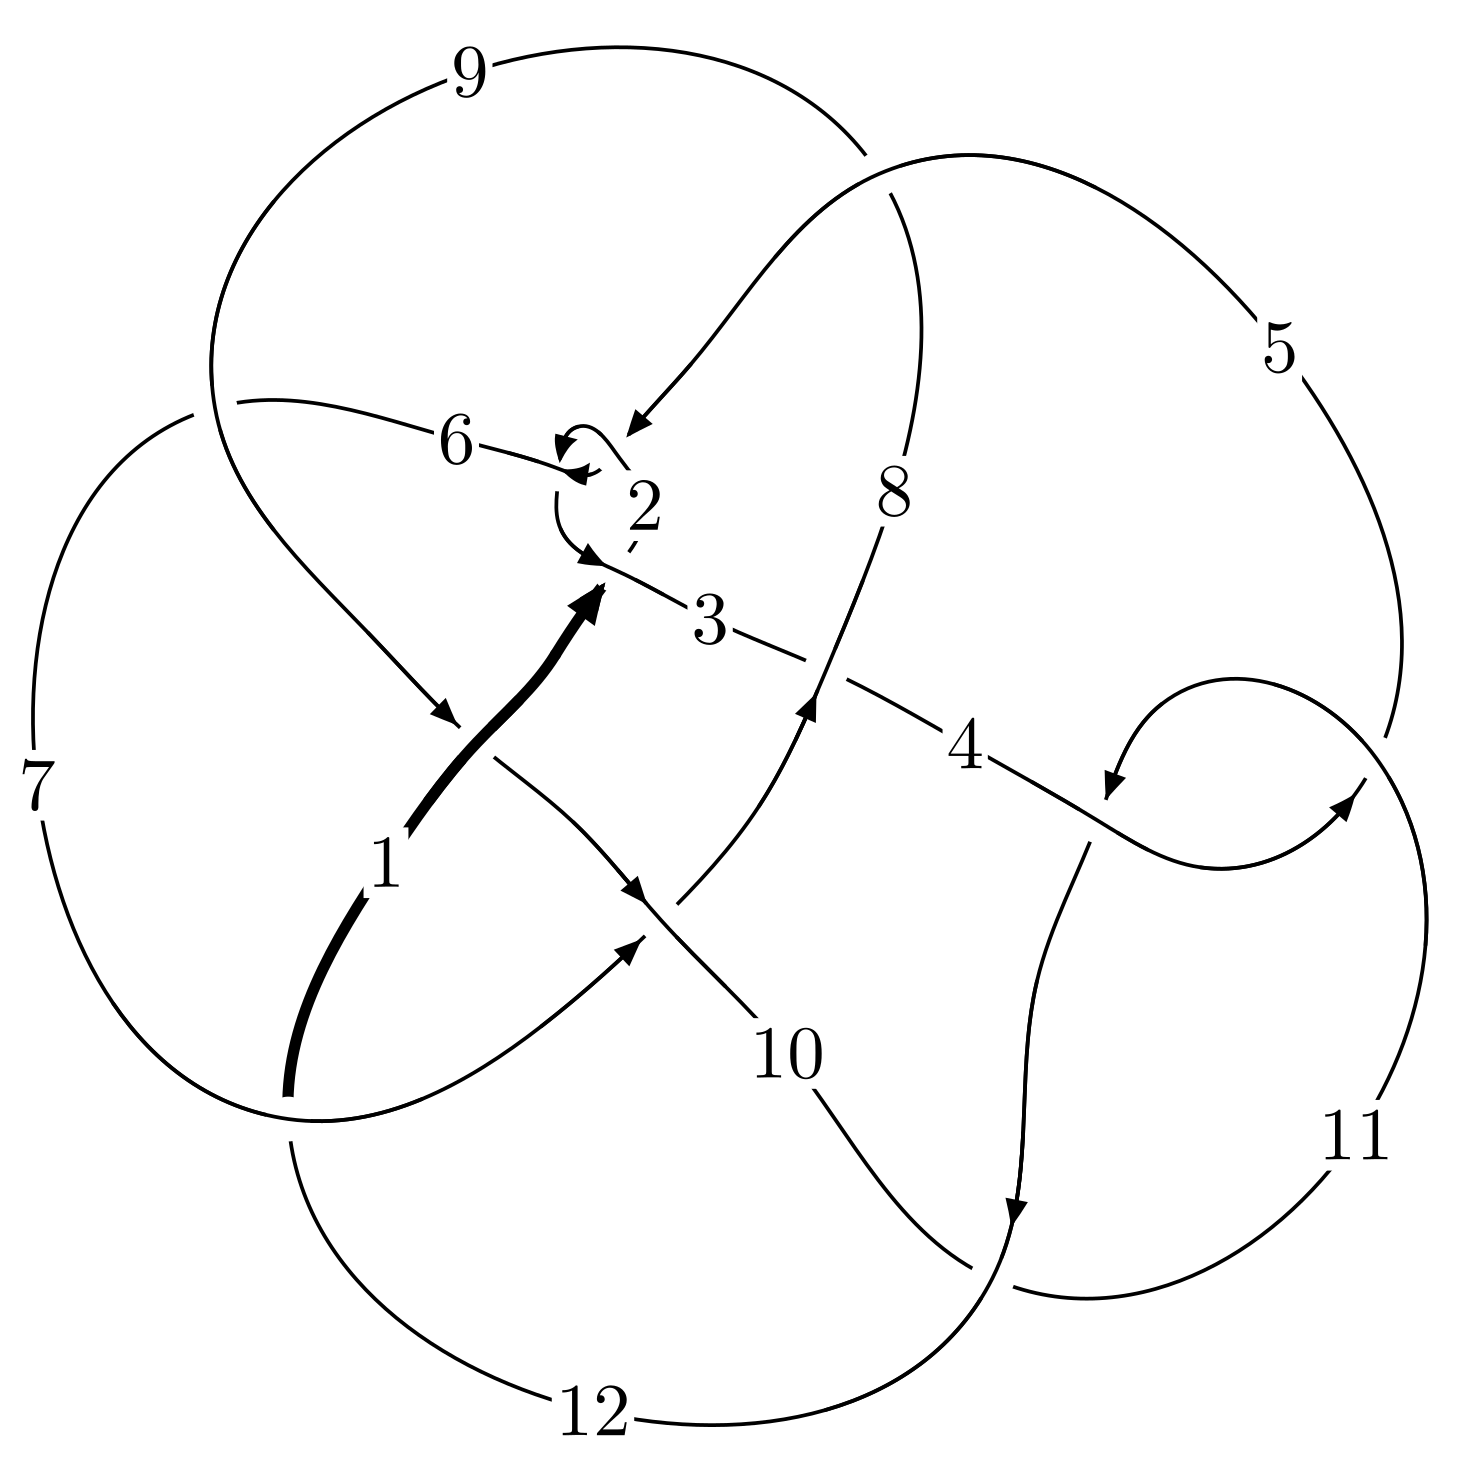
\includegraphics[width=112pt]{../../../GIT/diagram.site/Diagrams/png/1117_12a_0316.png}\\
\ \ \ A knot diagram\footnotemark}&
\allowdisplaybreaks
\textbf{Linearized knot diagam} \\
\cline{2-2}
 &
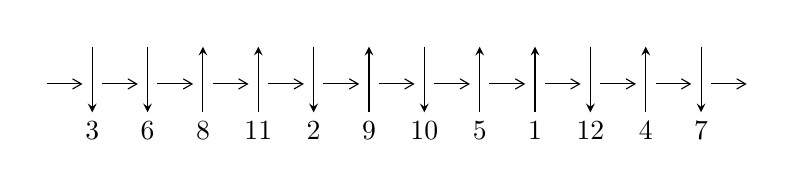
\begin{tikzpicture}[x=20pt, y=17pt]
	% nodes
	\node (C0) at (0, 0) {};
	\node (C1) at (1, 0) {};
	\node (C1U) at (1, +1) {};
	\node (C1D) at (1, -1) {3};

	\node (C2) at (2, 0) {};
	\node (C2U) at (2, +1) {};
	\node (C2D) at (2, -1) {6};

	\node (C3) at (3, 0) {};
	\node (C3U) at (3, +1) {};
	\node (C3D) at (3, -1) {8};

	\node (C4) at (4, 0) {};
	\node (C4U) at (4, +1) {};
	\node (C4D) at (4, -1) {11};

	\node (C5) at (5, 0) {};
	\node (C5U) at (5, +1) {};
	\node (C5D) at (5, -1) {2};

	\node (C6) at (6, 0) {};
	\node (C6U) at (6, +1) {};
	\node (C6D) at (6, -1) {9};

	\node (C7) at (7, 0) {};
	\node (C7U) at (7, +1) {};
	\node (C7D) at (7, -1) {10};

	\node (C8) at (8, 0) {};
	\node (C8U) at (8, +1) {};
	\node (C8D) at (8, -1) {5};

	\node (C9) at (9, 0) {};
	\node (C9U) at (9, +1) {};
	\node (C9D) at (9, -1) {1};

	\node (C10) at (10, 0) {};
	\node (C10U) at (10, +1) {};
	\node (C10D) at (10, -1) {12};

	\node (C11) at (11, 0) {};
	\node (C11U) at (11, +1) {};
	\node (C11D) at (11, -1) {4};

	\node (C12) at (12, 0) {};
	\node (C12U) at (12, +1) {};
	\node (C12D) at (12, -1) {7};
	\node (C13) at (13, 0) {};

	% arrows
	\draw[->,>={angle 60}]
	(C0) edge (C1) (C1) edge (C2) (C2) edge (C3) (C3) edge (C4) (C4) edge (C5) (C5) edge (C6) (C6) edge (C7) (C7) edge (C8) (C8) edge (C9) (C9) edge (C10) (C10) edge (C11) (C11) edge (C12) (C12) edge (C13) ;	\draw[->,>=stealth]
	(C1U) edge (C1D) (C2U) edge (C2D) (C3D) edge (C3U) (C4D) edge (C4U) (C5U) edge (C5D) (C6D) edge (C6U) (C7U) edge (C7D) (C8D) edge (C8U) (C9D) edge (C9U) (C10U) edge (C10D) (C11D) edge (C11U) (C12U) edge (C12D) ;
	\end{tikzpicture} \\
\hhline{~~} \\& 
\textbf{Solving Sequence} \\ \cline{2-2} 
 &
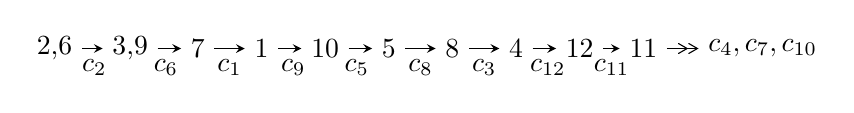
\begin{tikzpicture}[x=23pt, y=7pt]
	% node
	\node (A0) at (-1/8, 0) {2,6};
	\node (A1) at (17/16, 0) {3,9};
	\node (A2) at (17/8, 0) {7};
	\node (A3) at (25/8, 0) {1};
	\node (A4) at (33/8, 0) {10};
	\node (A5) at (41/8, 0) {5};
	\node (A6) at (49/8, 0) {8};
	\node (A7) at (57/8, 0) {4};
	\node (A8) at (65/8, 0) {12};
	\node (A9) at (73/8, 0) {11};
	\node (C1) at (1/2, -1) {$c_{2}$};
	\node (C2) at (13/8, -1) {$c_{6}$};
	\node (C3) at (21/8, -1) {$c_{1}$};
	\node (C4) at (29/8, -1) {$c_{9}$};
	\node (C5) at (37/8, -1) {$c_{5}$};
	\node (C6) at (45/8, -1) {$c_{8}$};
	\node (C7) at (53/8, -1) {$c_{3}$};
	\node (C8) at (61/8, -1) {$c_{12}$};
	\node (C9) at (69/8, -1) {$c_{11}$};
	\node (A10) at (11, 0) {$c_{4},c_{7},c_{10}$};

	% edge
	\draw[->,>=stealth]	
	(A0) edge (A1) (A1) edge (A2) (A2) edge (A3) (A3) edge (A4) (A4) edge (A5) (A5) edge (A6) (A6) edge (A7) (A7) edge (A8) (A8) edge (A9) ;
	\draw[->>,>={angle 60}]	
	(A9) edge (A10);
\end{tikzpicture} \\ 

\end{tabular} \\

\footnotetext{
The image of knot diagram is generated by the software ``\textbf{Draw programme}" developed by Andrew Bartholomew(\url{http://www.layer8.co.uk/maths/draw/index.htm\#Running-draw}), where we modified some parts for our purpose(\url{https://github.com/CATsTAILs/LinksPainter}).
}\phantom \\ \newline 
\centering \textbf{Ideals for irreducible components\footnotemark of $X_{\text{par}}$} 
 
\begin{align*}
I^u_{1}&=\langle 
6.27132\times10^{469} u^{176}+1.45967\times10^{471} u^{175}+\cdots+6.67248\times10^{470} b+1.46517\times10^{471},\\
\phantom{I^u_{1}}&\phantom{= \langle  }4.71016\times10^{471} u^{176}+1.68292\times10^{472} u^{175}+\cdots+6.67248\times10^{470} a+1.35006\times10^{472},\\
\phantom{I^u_{1}}&\phantom{= \langle  }u^{177}+4 u^{176}+\cdots+10 u+1\rangle \\
I^u_{2}&=\langle 
3206229 u^{36}-851287 u^{35}+\cdots+53147 b-2921496,\\
\phantom{I^u_{2}}&\phantom{= \langle  }3206229 u^{36}-851287 u^{35}+\cdots+53147 a-3134084,\;u^{37}+u^{36}+\cdots+2 u-1\rangle \\
\\
\end{align*}
\raggedright * 2 irreducible components of $\dim_{\mathbb{C}}=0$, with total 214 representations.\\
\footnotetext{All coefficients of polynomials are rational numbers. But the coefficients are sometimes approximated in decimal forms when there is not enough margin.}
\newpage
\renewcommand{\arraystretch}{1}
\centering \section*{I. $I^u_{1}= \langle 6.27\times10^{469} u^{176}+1.46\times10^{471} u^{175}+\cdots+6.67\times10^{470} b+1.47\times10^{471},\;4.71\times10^{471} u^{176}+1.68\times10^{472} u^{175}+\cdots+6.67\times10^{470} a+1.35\times10^{472},\;u^{177}+4 u^{176}+\cdots+10 u+1 \rangle$}
\flushleft \textbf{(i) Arc colorings}\\
\begin{tabular}{m{7pt} m{180pt} m{7pt} m{180pt} }
\flushright $a_{2}=$&$\begin{pmatrix}1\\0\end{pmatrix}$ \\
\flushright $a_{6}=$&$\begin{pmatrix}0\\u\end{pmatrix}$ \\
\flushright $a_{3}=$&$\begin{pmatrix}1\\u^2\end{pmatrix}$ \\
\flushright $a_{9}=$&$\begin{pmatrix}-7.05907 u^{176}-25.2217 u^{175}+\cdots-135.362 u-20.2332\\-0.0939879 u^{176}-2.18760 u^{175}+\cdots-25.6168 u-2.19583\end{pmatrix}$ \\
\flushright $a_{7}=$&$\begin{pmatrix}-1.26084 u^{176}-3.18185 u^{175}+\cdots+0.522136 u+4.94160\\-1.02841 u^{176}-2.49536 u^{175}+\cdots+7.10073 u+1.76271\end{pmatrix}$ \\
\flushright $a_{1}=$&$\begin{pmatrix}- u^2+1\\- u^4\end{pmatrix}$ \\
\flushright $a_{10}=$&$\begin{pmatrix}-11.7961 u^{176}-40.9296 u^{175}+\cdots-191.660 u-25.4602\\-4.25227 u^{176}-15.3984 u^{175}+\cdots-63.4411 u-6.27080\end{pmatrix}$ \\
\flushright $a_{5}=$&$\begin{pmatrix}u\\u\end{pmatrix}$ \\
\flushright $a_{8}=$&$\begin{pmatrix}-10.8853 u^{176}-37.9312 u^{175}+\cdots-176.659 u-25.0594\\-3.92024 u^{176}-14.8971 u^{175}+\cdots-66.9138 u-7.02204\end{pmatrix}$ \\
\flushright $a_{4}=$&$\begin{pmatrix}5.45380 u^{176}+22.5815 u^{175}+\cdots+155.803 u+18.4036\\-3.53508 u^{176}-8.38983 u^{175}+\cdots-20.8326 u-2.85652\end{pmatrix}$ \\
\flushright $a_{12}=$&$\begin{pmatrix}-2.20492 u^{176}-9.94931 u^{175}+\cdots-123.233 u-13.6295\\3.43657 u^{176}+12.3261 u^{175}+\cdots+48.1433 u+6.89118\end{pmatrix}$ \\
\flushright $a_{11}=$&$\begin{pmatrix}-14.5338 u^{176}-46.8491 u^{175}+\cdots-189.484 u-18.3827\\-7.41726 u^{176}-23.1558 u^{175}+\cdots-69.7149 u-6.96208\end{pmatrix}$\\&\end{tabular}
\flushleft \textbf{(ii) Obstruction class $= -1$}\\~\\
\flushleft \textbf{(iii) Cusp Shapes $= -18.8317 u^{176}-63.9674 u^{175}+\cdots-313.568 u-37.3249$}\\~\\
\newpage\renewcommand{\arraystretch}{1}
\flushleft \textbf{(iv) u-Polynomials at the component}\newline \\
\begin{tabular}{m{50pt}|m{274pt}}
Crossings & \hspace{64pt}u-Polynomials at each crossing \\
\hline $$\begin{aligned}c_{1}\end{aligned}$$&$\begin{aligned}
&u^{177}+80 u^{176}+\cdots+34 u+1
\end{aligned}$\\
\hline $$\begin{aligned}c_{2},c_{5}\end{aligned}$$&$\begin{aligned}
&u^{177}+4 u^{176}+\cdots+10 u+1
\end{aligned}$\\
\hline $$\begin{aligned}c_{3}\end{aligned}$$&$\begin{aligned}
&u^{177}+u^{176}+\cdots+220952 u-6793
\end{aligned}$\\
\hline $$\begin{aligned}c_{4},c_{11}\end{aligned}$$&$\begin{aligned}
&u^{177}+36 u^{175}+\cdots-195 u+59
\end{aligned}$\\
\hline $$\begin{aligned}c_{6}\end{aligned}$$&$\begin{aligned}
&u^{177}-17 u^{176}+\cdots-962894 u+202189
\end{aligned}$\\
\hline $$\begin{aligned}c_{7}\end{aligned}$$&$\begin{aligned}
&u^{177}+8 u^{176}+\cdots+79 u-1
\end{aligned}$\\
\hline $$\begin{aligned}c_{8}\end{aligned}$$&$\begin{aligned}
&u^{177}+u^{176}+\cdots-377547059 u-63518701
\end{aligned}$\\
\hline $$\begin{aligned}c_{9}\end{aligned}$$&$\begin{aligned}
&u^{177}+18 u^{176}+\cdots-5792 u-523
\end{aligned}$\\
\hline $$\begin{aligned}c_{10}\end{aligned}$$&$\begin{aligned}
&u^{177}+72 u^{176}+\cdots-103103 u-3481
\end{aligned}$\\
\hline $$\begin{aligned}c_{12}\end{aligned}$$&$\begin{aligned}
&u^{177}+5 u^{176}+\cdots+895865 u-154903
\end{aligned}$\\
\hline
\end{tabular}\\~\\
\newpage\renewcommand{\arraystretch}{1}
\flushleft \textbf{(v) Riley Polynomials at the component}\newline \\
\begin{tabular}{m{50pt}|m{274pt}}
Crossings & \hspace{64pt}Riley Polynomials at each crossing \\
\hline $$\begin{aligned}c_{1}\end{aligned}$$&$\begin{aligned}
&y^{177}+44 y^{176}+\cdots-2218 y-1
\end{aligned}$\\
\hline $$\begin{aligned}c_{2},c_{5}\end{aligned}$$&$\begin{aligned}
&y^{177}-80 y^{176}+\cdots+34 y-1
\end{aligned}$\\
\hline $$\begin{aligned}c_{3}\end{aligned}$$&$\begin{aligned}
&y^{177}-17 y^{176}+\cdots+37538868580 y-46144849
\end{aligned}$\\
\hline $$\begin{aligned}c_{4},c_{11}\end{aligned}$$&$\begin{aligned}
&y^{177}+72 y^{176}+\cdots-103103 y-3481
\end{aligned}$\\
\hline $$\begin{aligned}c_{6}\end{aligned}$$&$\begin{aligned}
&y^{177}-27 y^{176}+\cdots-44453979886 y-40880391721
\end{aligned}$\\
\hline $$\begin{aligned}c_{7}\end{aligned}$$&$\begin{aligned}
&y^{177}+12 y^{176}+\cdots+549 y-1
\end{aligned}$\\
\hline $$\begin{aligned}c_{8}\end{aligned}$$&$\begin{aligned}
&y^{177}-37 y^{176}+\cdots+270860312130815791 y-4034625376727401
\end{aligned}$\\
\hline $$\begin{aligned}c_{9}\end{aligned}$$&$\begin{aligned}
&y^{177}+8 y^{176}+\cdots-28982616 y-273529
\end{aligned}$\\
\hline $$\begin{aligned}c_{10}\end{aligned}$$&$\begin{aligned}
&y^{177}+72 y^{176}+\cdots-1149837415 y-12117361
\end{aligned}$\\
\hline $$\begin{aligned}c_{12}\end{aligned}$$&$\begin{aligned}
&y^{177}+31 y^{176}+\cdots-1661817074137 y-23994939409
\end{aligned}$\\
\hline
\end{tabular}\\~\\
\newpage\flushleft \textbf{(vi) Complex Volumes and Cusp Shapes}
$$\begin{array}{c|c|c}  
\text{Solutions to }I^u_{1}& \I (\text{vol} + \sqrt{-1}CS) & \text{Cusp shape}\\
 \hline 
\begin{aligned}
u &= \phantom{-}0.864110 + 0.503380 I \\
a &= \phantom{-}1.64210 - 0.28849 I \\
b &= \phantom{-}0.453580 + 0.130110 I\end{aligned}
 & \phantom{-}3.02236 + 0.80080 I & \phantom{-0.000000 } 0 \\ \hline\begin{aligned}
u &= \phantom{-}0.864110 - 0.503380 I \\
a &= \phantom{-}1.64210 + 0.28849 I \\
b &= \phantom{-}0.453580 - 0.130110 I\end{aligned}
 & \phantom{-}3.02236 - 0.80080 I & \phantom{-0.000000 } 0 \\ \hline\begin{aligned}
u &= \phantom{-}0.854454 + 0.530174 I \\
a &= \phantom{-}0.581132 - 1.206900 I \\
b &= \phantom{-}1.18512 - 2.00320 I\end{aligned}
 & \phantom{-}3.02605 - 4.97258 I & \phantom{-0.000000 } 0 \\ \hline\begin{aligned}
u &= \phantom{-}0.854454 - 0.530174 I \\
a &= \phantom{-}0.581132 + 1.206900 I \\
b &= \phantom{-}1.18512 + 2.00320 I\end{aligned}
 & \phantom{-}3.02605 + 4.97258 I & \phantom{-0.000000 } 0 \\ \hline\begin{aligned}
u &= \phantom{-}0.628733 + 0.785612 I \\
a &= -0.722882 + 0.572565 I \\
b &= \phantom{-}0.538006 - 0.109119 I\end{aligned}
 & \phantom{-}6.22275 + 0.33470 I & \phantom{-0.000000 } 0 \\ \hline\begin{aligned}
u &= \phantom{-}0.628733 - 0.785612 I \\
a &= -0.722882 - 0.572565 I \\
b &= \phantom{-}0.538006 + 0.109119 I\end{aligned}
 & \phantom{-}6.22275 - 0.33470 I & \phantom{-0.000000 } 0 \\ \hline\begin{aligned}
u &= -0.995131 + 0.150101 I \\
a &= -0.730128 + 0.587590 I \\
b &= -1.69476 + 1.26240 I\end{aligned}
 & \phantom{-}0.137829 + 1.011590 I & \phantom{-0.000000 } 0 \\ \hline\begin{aligned}
u &= -0.995131 - 0.150101 I \\
a &= -0.730128 - 0.587590 I \\
b &= -1.69476 - 1.26240 I\end{aligned}
 & \phantom{-}0.137829 - 1.011590 I & \phantom{-0.000000 } 0 \\ \hline\begin{aligned}
u &= \phantom{-}0.429828 + 0.910229 I \\
a &= -1.26729 + 0.89068 I \\
b &= -0.0504466 + 0.0116262 I\end{aligned}
 & \phantom{-}5.31765 + 9.00835 I & \phantom{-0.000000 } 0 \\ \hline\begin{aligned}
u &= \phantom{-}0.429828 - 0.910229 I \\
a &= -1.26729 - 0.89068 I \\
b &= -0.0504466 - 0.0116262 I\end{aligned}
 & \phantom{-}5.31765 - 9.00835 I & \phantom{-0.000000 } 0\\
 \hline 
 \end{array}$$\newpage$$\begin{array}{c|c|c}  
\text{Solutions to }I^u_{1}& \I (\text{vol} + \sqrt{-1}CS) & \text{Cusp shape}\\
 \hline 
\begin{aligned}
u &= -0.431978 + 0.909727 I \\
a &= \phantom{-}1.099430 + 0.678193 I \\
b &= -0.0703223 + 0.1208490 I\end{aligned}
 & -1.84822 - 7.07977 I & \phantom{-0.000000 } 0 \\ \hline\begin{aligned}
u &= -0.431978 - 0.909727 I \\
a &= \phantom{-}1.099430 - 0.678193 I \\
b &= -0.0703223 - 0.1208490 I\end{aligned}
 & -1.84822 + 7.07977 I & \phantom{-0.000000 } 0 \\ \hline\begin{aligned}
u &= -0.430940 + 0.912090 I \\
a &= \phantom{-}1.35273 + 0.84882 I \\
b &= \phantom{-}0.0209828 - 0.0429838 I\end{aligned}
 & \phantom{-}3.6105 - 15.0225 I & \phantom{-0.000000 } 0 \\ \hline\begin{aligned}
u &= -0.430940 - 0.912090 I \\
a &= \phantom{-}1.35273 - 0.84882 I \\
b &= \phantom{-}0.0209828 + 0.0429838 I\end{aligned}
 & \phantom{-}3.6105 + 15.0225 I & \phantom{-0.000000 } 0 \\ \hline\begin{aligned}
u &= -0.689258 + 0.741416 I \\
a &= -1.51421 - 0.54650 I \\
b &= -0.990121 - 0.092074 I\end{aligned}
 & \phantom{-}4.35698 + 0.21526 I & \phantom{-0.000000 } 0 \\ \hline\begin{aligned}
u &= -0.689258 - 0.741416 I \\
a &= -1.51421 + 0.54650 I \\
b &= -0.990121 + 0.092074 I\end{aligned}
 & \phantom{-}4.35698 - 0.21526 I & \phantom{-0.000000 } 0 \\ \hline\begin{aligned}
u &= -0.983063 + 0.244776 I \\
a &= \phantom{-}0.086827 - 0.874000 I \\
b &= -0.92991 - 1.40928 I\end{aligned}
 & -3.69375 + 1.07233 I & \phantom{-0.000000 } 0 \\ \hline\begin{aligned}
u &= -0.983063 - 0.244776 I \\
a &= \phantom{-}0.086827 + 0.874000 I \\
b &= -0.92991 + 1.40928 I\end{aligned}
 & -3.69375 - 1.07233 I & \phantom{-0.000000 } 0 \\ \hline\begin{aligned}
u &= \phantom{-}0.556234 + 0.847392 I \\
a &= \phantom{-}1.232020 - 0.344639 I \\
b &= \phantom{-}0.306913 + 0.299878 I\end{aligned}
 & \phantom{-}2.34667 + 1.51020 I & \phantom{-0.000000 } 0 \\ \hline\begin{aligned}
u &= \phantom{-}0.556234 - 0.847392 I \\
a &= \phantom{-}1.232020 + 0.344639 I \\
b &= \phantom{-}0.306913 - 0.299878 I\end{aligned}
 & \phantom{-}2.34667 - 1.51020 I & \phantom{-0.000000 } 0\\
 \hline 
 \end{array}$$\newpage$$\begin{array}{c|c|c}  
\text{Solutions to }I^u_{1}& \I (\text{vol} + \sqrt{-1}CS) & \text{Cusp shape}\\
 \hline 
\begin{aligned}
u &= -0.814374 + 0.549309 I \\
a &= -0.779171 - 0.971826 I \\
b &= -1.14533 - 1.70016 I\end{aligned}
 & \phantom{-}3.39876 - 0.49100 I & \phantom{-0.000000 } 0 \\ \hline\begin{aligned}
u &= -0.814374 - 0.549309 I \\
a &= -0.779171 + 0.971826 I \\
b &= -1.14533 + 1.70016 I\end{aligned}
 & \phantom{-}3.39876 + 0.49100 I & \phantom{-0.000000 } 0 \\ \hline\begin{aligned}
u &= -0.880785 + 0.526592 I \\
a &= -1.42262 - 0.63982 I \\
b &= -0.325054 - 0.362166 I\end{aligned}
 & \phantom{-}3.20866 + 4.81840 I & \phantom{-0.000000 } 0 \\ \hline\begin{aligned}
u &= -0.880785 - 0.526592 I \\
a &= -1.42262 + 0.63982 I \\
b &= -0.325054 + 0.362166 I\end{aligned}
 & \phantom{-}3.20866 - 4.81840 I & \phantom{-0.000000 } 0 \\ \hline\begin{aligned}
u &= \phantom{-}0.673023 + 0.777597 I \\
a &= \phantom{-}1.54096 - 0.46393 I \\
b &= \phantom{-}0.891807 + 0.136620 I\end{aligned}
 & \phantom{-}4.16997 + 4.65462 I & \phantom{-0.000000 } 0 \\ \hline\begin{aligned}
u &= \phantom{-}0.673023 - 0.777597 I \\
a &= \phantom{-}1.54096 + 0.46393 I \\
b &= \phantom{-}0.891807 - 0.136620 I\end{aligned}
 & \phantom{-}4.16997 - 4.65462 I & \phantom{-0.000000 } 0 \\ \hline\begin{aligned}
u &= \phantom{-}1.016800 + 0.178760 I \\
a &= \phantom{-}0.839498 + 0.723029 I \\
b &= \phantom{-}1.74110 + 1.69079 I\end{aligned}
 & -0.10196 + 3.78125 I & \phantom{-0.000000 } 0 \\ \hline\begin{aligned}
u &= \phantom{-}1.016800 - 0.178760 I \\
a &= \phantom{-}0.839498 - 0.723029 I \\
b &= \phantom{-}1.74110 - 1.69079 I\end{aligned}
 & -0.10196 - 3.78125 I & \phantom{-0.000000 } 0 \\ \hline\begin{aligned}
u &= \phantom{-}0.413682 + 0.948840 I \\
a &= -0.745949 + 0.906108 I \\
b &= -0.053103 + 0.298477 I\end{aligned}
 & \phantom{-}4.35149 + 3.60655 I & \phantom{-0.000000 } 0 \\ \hline\begin{aligned}
u &= \phantom{-}0.413682 - 0.948840 I \\
a &= -0.745949 - 0.906108 I \\
b &= -0.053103 - 0.298477 I\end{aligned}
 & \phantom{-}4.35149 - 3.60655 I & \phantom{-0.000000 } 0\\
 \hline 
 \end{array}$$\newpage$$\begin{array}{c|c|c}  
\text{Solutions to }I^u_{1}& \I (\text{vol} + \sqrt{-1}CS) & \text{Cusp shape}\\
 \hline 
\begin{aligned}
u &= \phantom{-}0.993594 + 0.291384 I \\
a &= \phantom{-}0.844216 + 0.946999 I \\
b &= \phantom{-}0.93027 + 2.29117 I\end{aligned}
 & -1.66504 + 0.52353 I & \phantom{-0.000000 } 0 \\ \hline\begin{aligned}
u &= \phantom{-}0.993594 - 0.291384 I \\
a &= \phantom{-}0.844216 - 0.946999 I \\
b &= \phantom{-}0.93027 - 2.29117 I\end{aligned}
 & -1.66504 - 0.52353 I & \phantom{-0.000000 } 0 \\ \hline\begin{aligned}
u &= \phantom{-}0.895649 + 0.357166 I \\
a &= \phantom{-}1.025610 + 0.918358 I \\
b &= \phantom{-}0.45506 + 1.74939 I\end{aligned}
 & -1.23431 + 0.87708 I & \phantom{-0.000000 } 0 \\ \hline\begin{aligned}
u &= \phantom{-}0.895649 - 0.357166 I \\
a &= \phantom{-}1.025610 - 0.918358 I \\
b &= \phantom{-}0.45506 - 1.74939 I\end{aligned}
 & -1.23431 - 0.87708 I & \phantom{-0.000000 } 0 \\ \hline\begin{aligned}
u &= -0.605031 + 0.748752 I \\
a &= \phantom{-}0.843894 + 0.498704 I \\
b &= -0.709249 - 0.239796 I\end{aligned}
 & \phantom{-}4.30109 - 6.39022 I & \phantom{-0.000000 } 0 \\ \hline\begin{aligned}
u &= -0.605031 - 0.748752 I \\
a &= \phantom{-}0.843894 - 0.498704 I \\
b &= -0.709249 + 0.239796 I\end{aligned}
 & \phantom{-}4.30109 + 6.39022 I & \phantom{-0.000000 } 0 \\ \hline\begin{aligned}
u &= \phantom{-}0.966875 + 0.380234 I \\
a &= -0.52633 + 1.66575 I \\
b &= \phantom{-}0.39230 + 2.53238 I\end{aligned}
 & -2.02402 + 4.85256 I & \phantom{-0.000000 } 0 \\ \hline\begin{aligned}
u &= \phantom{-}0.966875 - 0.380234 I \\
a &= -0.52633 - 1.66575 I \\
b &= \phantom{-}0.39230 - 2.53238 I\end{aligned}
 & -2.02402 - 4.85256 I & \phantom{-0.000000 } 0 \\ \hline\begin{aligned}
u &= -0.969471 + 0.379442 I \\
a &= \phantom{-}0.287010 + 1.361120 I \\
b &= -0.58379 + 2.08508 I\end{aligned}
 & -0.854958 + 0.471035 I & \phantom{-0.000000 } 0 \\ \hline\begin{aligned}
u &= -0.969471 - 0.379442 I \\
a &= \phantom{-}0.287010 - 1.361120 I \\
b &= -0.58379 - 2.08508 I\end{aligned}
 & -0.854958 - 0.471035 I & \phantom{-0.000000 } 0\\
 \hline 
 \end{array}$$\newpage$$\begin{array}{c|c|c}  
\text{Solutions to }I^u_{1}& \I (\text{vol} + \sqrt{-1}CS) & \text{Cusp shape}\\
 \hline 
\begin{aligned}
u &= -0.334151 + 0.990251 I \\
a &= -0.463534 - 0.392409 I \\
b &= -0.004647 + 0.230446 I\end{aligned}
 & -0.814141 + 0.510005 I & \phantom{-0.000000 } 0 \\ \hline\begin{aligned}
u &= -0.334151 - 0.990251 I \\
a &= -0.463534 + 0.392409 I \\
b &= -0.004647 - 0.230446 I\end{aligned}
 & -0.814141 - 0.510005 I & \phantom{-0.000000 } 0 \\ \hline\begin{aligned}
u &= \phantom{-}0.981019 + 0.368545 I \\
a &= -1.02461 + 0.98094 I \\
b &= -0.46481 + 1.88356 I\end{aligned}
 & -6.14172 - 1.19459 I & \phantom{-0.000000 } 0 \\ \hline\begin{aligned}
u &= \phantom{-}0.981019 - 0.368545 I \\
a &= -1.02461 - 0.98094 I \\
b &= -0.46481 - 1.88356 I\end{aligned}
 & -6.14172 + 1.19459 I & \phantom{-0.000000 } 0 \\ \hline\begin{aligned}
u &= -0.954229 + 0.434373 I \\
a &= -0.738335 + 0.615680 I \\
b &= \phantom{-}0.40593 + 2.03400 I\end{aligned}
 & -4.50486 + 1.86213 I & \phantom{-0.000000 } 0 \\ \hline\begin{aligned}
u &= -0.954229 - 0.434373 I \\
a &= -0.738335 - 0.615680 I \\
b &= \phantom{-}0.40593 - 2.03400 I\end{aligned}
 & -4.50486 - 1.86213 I & \phantom{-0.000000 } 0 \\ \hline\begin{aligned}
u &= \phantom{-}0.482512 + 0.810071 I \\
a &= \phantom{-}1.120650 - 0.605325 I \\
b &= \phantom{-}0.180308 + 0.169055 I\end{aligned}
 & \phantom{-}2.43714 + 1.63530 I & \phantom{-0.000000 } 0 \\ \hline\begin{aligned}
u &= \phantom{-}0.482512 - 0.810071 I \\
a &= \phantom{-}1.120650 + 0.605325 I \\
b &= \phantom{-}0.180308 - 0.169055 I\end{aligned}
 & \phantom{-}2.43714 - 1.63530 I & \phantom{-0.000000 } 0 \\ \hline\begin{aligned}
u &= \phantom{-}0.968611 + 0.427868 I \\
a &= -0.466538 - 0.976942 I \\
b &= \phantom{-}0.23731 - 1.57700 I\end{aligned}
 & -1.71516 - 3.91586 I & \phantom{-0.000000 } 0 \\ \hline\begin{aligned}
u &= \phantom{-}0.968611 - 0.427868 I \\
a &= -0.466538 + 0.976942 I \\
b &= \phantom{-}0.23731 + 1.57700 I\end{aligned}
 & -1.71516 + 3.91586 I & \phantom{-0.000000 } 0\\
 \hline 
 \end{array}$$\newpage$$\begin{array}{c|c|c}  
\text{Solutions to }I^u_{1}& \I (\text{vol} + \sqrt{-1}CS) & \text{Cusp shape}\\
 \hline 
\begin{aligned}
u &= -1.007150 + 0.358789 I \\
a &= -0.779760 + 0.932037 I \\
b &= -0.41402 + 2.57889 I\end{aligned}
 & -2.82839 - 4.64321 I & \phantom{-0.000000 } 0 \\ \hline\begin{aligned}
u &= -1.007150 - 0.358789 I \\
a &= -0.779760 - 0.932037 I \\
b &= -0.41402 - 2.57889 I\end{aligned}
 & -2.82839 + 4.64321 I & \phantom{-0.000000 } 0 \\ \hline\begin{aligned}
u &= \phantom{-}0.953295 + 0.486416 I \\
a &= \phantom{-}0.397010 - 0.541125 I \\
b &= -1.47341 - 1.50063 I\end{aligned}
 & -4.20211 - 3.46738 I & \phantom{-0.000000 } 0 \\ \hline\begin{aligned}
u &= \phantom{-}0.953295 - 0.486416 I \\
a &= \phantom{-}0.397010 + 0.541125 I \\
b &= -1.47341 + 1.50063 I\end{aligned}
 & -4.20211 + 3.46738 I & \phantom{-0.000000 } 0 \\ \hline\begin{aligned}
u &= -0.533783 + 0.934684 I \\
a &= -0.976099 - 0.139686 I \\
b &= -0.106331 + 0.396116 I\end{aligned}
 & \phantom{-}1.03900 - 5.79820 I & \phantom{-0.000000 } 0 \\ \hline\begin{aligned}
u &= -0.533783 - 0.934684 I \\
a &= -0.976099 + 0.139686 I \\
b &= -0.106331 - 0.396116 I\end{aligned}
 & \phantom{-}1.03900 + 5.79820 I & \phantom{-0.000000 } 0 \\ \hline\begin{aligned}
u &= -0.981695 + 0.447205 I \\
a &= \phantom{-}0.364521 + 0.474478 I \\
b &= -0.228931 + 1.035680 I\end{aligned}
 & -1.59398 + 1.86715 I & \phantom{-0.000000 } 0 \\ \hline\begin{aligned}
u &= -0.981695 - 0.447205 I \\
a &= \phantom{-}0.364521 - 0.474478 I \\
b &= -0.228931 - 1.035680 I\end{aligned}
 & -1.59398 - 1.86715 I & \phantom{-0.000000 } 0 \\ \hline\begin{aligned}
u &= -0.686189 + 0.838109 I \\
a &= \phantom{-}0.422512 + 0.531598 I \\
b &= -0.115585 + 0.289545 I\end{aligned}
 & -0.33435 + 2.65275 I & \phantom{-0.000000 } 0 \\ \hline\begin{aligned}
u &= -0.686189 - 0.838109 I \\
a &= \phantom{-}0.422512 - 0.531598 I \\
b &= -0.115585 - 0.289545 I\end{aligned}
 & -0.33435 - 2.65275 I & \phantom{-0.000000 } 0\\
 \hline 
 \end{array}$$\newpage$$\begin{array}{c|c|c}  
\text{Solutions to }I^u_{1}& \I (\text{vol} + \sqrt{-1}CS) & \text{Cusp shape}\\
 \hline 
\begin{aligned}
u &= \phantom{-}0.641662 + 0.873189 I \\
a &= -0.467333 + 0.778610 I \\
b &= \phantom{-}0.0584398 - 0.0639245 I\end{aligned}
 & \phantom{-}6.61970 - 4.57530 I & \phantom{-0.000000 } 0 \\ \hline\begin{aligned}
u &= \phantom{-}0.641662 - 0.873189 I \\
a &= -0.467333 - 0.778610 I \\
b &= \phantom{-}0.0584398 + 0.0639245 I\end{aligned}
 & \phantom{-}6.61970 + 4.57530 I & \phantom{-0.000000 } 0 \\ \hline\begin{aligned}
u &= \phantom{-}0.976335 + 0.497172 I \\
a &= -1.08695 - 1.54329 I \\
b &= -0.69036 - 2.42165 I\end{aligned}
 & -0.15175 - 5.18017 I & \phantom{-0.000000 } 0 \\ \hline\begin{aligned}
u &= \phantom{-}0.976335 - 0.497172 I \\
a &= -1.08695 + 1.54329 I \\
b &= -0.69036 + 2.42165 I\end{aligned}
 & -0.15175 + 5.18017 I & \phantom{-0.000000 } 0 \\ \hline\begin{aligned}
u &= -0.643816 + 0.892856 I \\
a &= \phantom{-}0.394328 + 0.823883 I \\
b &= \phantom{-}0.0398039 - 0.0652166 I\end{aligned}
 & \phantom{-}4.88923 + 10.48330 I & \phantom{-0.000000 } 0 \\ \hline\begin{aligned}
u &= -0.643816 - 0.892856 I \\
a &= \phantom{-}0.394328 - 0.823883 I \\
b &= \phantom{-}0.0398039 + 0.0652166 I\end{aligned}
 & \phantom{-}4.88923 - 10.48330 I & \phantom{-0.000000 } 0 \\ \hline\begin{aligned}
u &= -0.984038 + 0.507492 I \\
a &= \phantom{-}1.39816 - 1.54570 I \\
b &= \phantom{-}1.12239 - 2.46986 I\end{aligned}
 & -1.20216 + 10.51620 I & \phantom{-0.000000 } 0 \\ \hline\begin{aligned}
u &= -0.984038 - 0.507492 I \\
a &= \phantom{-}1.39816 + 1.54570 I \\
b &= \phantom{-}1.12239 + 2.46986 I\end{aligned}
 & -1.20216 - 10.51620 I & \phantom{-0.000000 } 0 \\ \hline\begin{aligned}
u &= \phantom{-}1.074180 + 0.314145 I \\
a &= -1.187290 + 0.107309 I \\
b &= -1.30256 + 0.80314 I\end{aligned}
 & -1.71410 - 6.86279 I & \phantom{-0.000000 } 0 \\ \hline\begin{aligned}
u &= \phantom{-}1.074180 - 0.314145 I \\
a &= -1.187290 - 0.107309 I \\
b &= -1.30256 - 0.80314 I\end{aligned}
 & -1.71410 + 6.86279 I & \phantom{-0.000000 } 0\\
 \hline 
 \end{array}$$\newpage$$\begin{array}{c|c|c}  
\text{Solutions to }I^u_{1}& \I (\text{vol} + \sqrt{-1}CS) & \text{Cusp shape}\\
 \hline 
\begin{aligned}
u &= -0.986129 + 0.529695 I \\
a &= -0.446989 - 0.969513 I \\
b &= \phantom{-}0.45388 - 2.03741 I\end{aligned}
 & \phantom{-}0.06124 + 6.22009 I & \phantom{-0.000000 } 0 \\ \hline\begin{aligned}
u &= -0.986129 - 0.529695 I \\
a &= -0.446989 + 0.969513 I \\
b &= \phantom{-}0.45388 + 2.03741 I\end{aligned}
 & \phantom{-}0.06124 - 6.22009 I & \phantom{-0.000000 } 0 \\ \hline\begin{aligned}
u &= \phantom{-}0.766407 + 0.418178 I \\
a &= \phantom{-}0.318503 - 0.142059 I \\
b &= -0.02476 - 2.36651 I\end{aligned}
 & -3.49282 - 0.33241 I & \phantom{-0.000000 } 0 \\ \hline\begin{aligned}
u &= \phantom{-}0.766407 - 0.418178 I \\
a &= \phantom{-}0.318503 + 0.142059 I \\
b &= -0.02476 + 2.36651 I\end{aligned}
 & -3.49282 + 0.33241 I & \phantom{-0.000000 } 0 \\ \hline\begin{aligned}
u &= \phantom{-}1.013210 + 0.498461 I \\
a &= \phantom{-}0.181595 - 0.942807 I \\
b &= -0.88594 - 2.57967 I\end{aligned}
 & -1.94333 - 10.80760 I & \phantom{-0.000000 } 0 \\ \hline\begin{aligned}
u &= \phantom{-}1.013210 - 0.498461 I \\
a &= \phantom{-}0.181595 + 0.942807 I \\
b &= -0.88594 + 2.57967 I\end{aligned}
 & -1.94333 + 10.80760 I & \phantom{-0.000000 } 0 \\ \hline\begin{aligned}
u &= -0.203869 + 0.844369 I \\
a &= \phantom{-}0.240509 + 1.358190 I \\
b &= \phantom{-}0.129274 + 0.558191 I\end{aligned}
 & \phantom{-}2.35834 + 3.63220 I & \phantom{-0.000000 } 0 \\ \hline\begin{aligned}
u &= -0.203869 - 0.844369 I \\
a &= \phantom{-}0.240509 - 1.358190 I \\
b &= \phantom{-}0.129274 - 0.558191 I\end{aligned}
 & \phantom{-}2.35834 - 3.63220 I & \phantom{-0.000000 } 0 \\ \hline\begin{aligned}
u &= -1.020510 + 0.488503 I \\
a &= \phantom{-}1.28197 - 0.78165 I \\
b &= \phantom{-}1.10918 - 1.32805 I\end{aligned}
 & -5.32571 + 4.91021 I & \phantom{-0.000000 } 0 \\ \hline\begin{aligned}
u &= -1.020510 - 0.488503 I \\
a &= \phantom{-}1.28197 + 0.78165 I \\
b &= \phantom{-}1.10918 + 1.32805 I\end{aligned}
 & -5.32571 - 4.91021 I & \phantom{-0.000000 } 0\\
 \hline 
 \end{array}$$\newpage$$\begin{array}{c|c|c}  
\text{Solutions to }I^u_{1}& \I (\text{vol} + \sqrt{-1}CS) & \text{Cusp shape}\\
 \hline 
\begin{aligned}
u &= \phantom{-}0.454584 + 0.720457 I \\
a &= \phantom{-}1.76325 - 0.93699 I \\
b &= \phantom{-}0.0092184 + 0.1017300 I\end{aligned}
 & \phantom{-}4.72116 + 0.61300 I & \phantom{-0.000000 } 0 \\ \hline\begin{aligned}
u &= \phantom{-}0.454584 - 0.720457 I \\
a &= \phantom{-}1.76325 + 0.93699 I \\
b &= \phantom{-}0.0092184 - 0.1017300 I\end{aligned}
 & \phantom{-}4.72116 - 0.61300 I & \phantom{-0.000000 } 0 \\ \hline\begin{aligned}
u &= -1.107280 + 0.360761 I \\
a &= -0.046154 - 0.532157 I \\
b &= -1.35787 - 0.75946 I\end{aligned}
 & -2.80776 + 5.90177 I & \phantom{-0.000000 } 0 \\ \hline\begin{aligned}
u &= -1.107280 - 0.360761 I \\
a &= -0.046154 + 0.532157 I \\
b &= -1.35787 + 0.75946 I\end{aligned}
 & -2.80776 - 5.90177 I & \phantom{-0.000000 } 0 \\ \hline\begin{aligned}
u &= -0.443082 + 0.704654 I \\
a &= -1.89935 - 0.78762 I \\
b &= \phantom{-}0.0903060 + 0.0571122 I\end{aligned}
 & \phantom{-}4.33274 - 5.54339 I & \phantom{-0.000000 } 0 \\ \hline\begin{aligned}
u &= -0.443082 - 0.704654 I \\
a &= -1.89935 + 0.78762 I \\
b &= \phantom{-}0.0903060 - 0.0571122 I\end{aligned}
 & \phantom{-}4.33274 + 5.54339 I & \phantom{-0.000000 } 0 \\ \hline\begin{aligned}
u &= -0.972572 + 0.650132 I \\
a &= -0.57392 - 1.55176 I \\
b &= -0.79279 - 1.91590 I\end{aligned}
 & \phantom{-}3.48309 + 5.08902 I & \phantom{-0.000000 } 0 \\ \hline\begin{aligned}
u &= -0.972572 - 0.650132 I \\
a &= -0.57392 + 1.55176 I \\
b &= -0.79279 + 1.91590 I\end{aligned}
 & \phantom{-}3.48309 - 5.08902 I & \phantom{-0.000000 } 0 \\ \hline\begin{aligned}
u &= \phantom{-}1.071370 + 0.472682 I \\
a &= -0.125573 + 0.151807 I \\
b &= \phantom{-}0.754288 + 0.695071 I\end{aligned}
 & -2.42037 - 5.73814 I & \phantom{-0.000000 } 0 \\ \hline\begin{aligned}
u &= \phantom{-}1.071370 - 0.472682 I \\
a &= -0.125573 - 0.151807 I \\
b &= \phantom{-}0.754288 - 0.695071 I\end{aligned}
 & -2.42037 + 5.73814 I & \phantom{-0.000000 } 0\\
 \hline 
 \end{array}$$\newpage$$\begin{array}{c|c|c}  
\text{Solutions to }I^u_{1}& \I (\text{vol} + \sqrt{-1}CS) & \text{Cusp shape}\\
 \hline 
\begin{aligned}
u &= \phantom{-}0.727816 + 0.388140 I \\
a &= \phantom{-}1.46503 + 1.79064 I \\
b &= \phantom{-}0.71399 + 1.66257 I\end{aligned}
 & \phantom{-}0.80530 + 1.36238 I & \phantom{-0.000000 } 0 \\ \hline\begin{aligned}
u &= \phantom{-}0.727816 - 0.388140 I \\
a &= \phantom{-}1.46503 - 1.79064 I \\
b &= \phantom{-}0.71399 - 1.66257 I\end{aligned}
 & \phantom{-}0.80530 - 1.36238 I & \phantom{-0.000000 } 0 \\ \hline\begin{aligned}
u &= -1.034940 + 0.566622 I \\
a &= -0.385371 - 1.274380 I \\
b &= -0.26876 - 2.61647 I\end{aligned}
 & \phantom{-}0.18035 + 6.67560 I & \phantom{-0.000000 } 0 \\ \hline\begin{aligned}
u &= -1.034940 - 0.566622 I \\
a &= -0.385371 + 1.274380 I \\
b &= -0.26876 + 2.61647 I\end{aligned}
 & \phantom{-}0.18035 - 6.67560 I & \phantom{-0.000000 } 0 \\ \hline\begin{aligned}
u &= \phantom{-}1.110490 + 0.400960 I \\
a &= \phantom{-}0.047678 - 0.338435 I \\
b &= \phantom{-}1.338290 - 0.291718 I\end{aligned}
 & -2.57340 - 1.75170 I & \phantom{-0.000000 } 0 \\ \hline\begin{aligned}
u &= \phantom{-}1.110490 - 0.400960 I \\
a &= \phantom{-}0.047678 + 0.338435 I \\
b &= \phantom{-}1.338290 + 0.291718 I\end{aligned}
 & -2.57340 + 1.75170 I & \phantom{-0.000000 } 0 \\ \hline\begin{aligned}
u &= -0.539683 + 0.613755 I \\
a &= -1.52577 - 0.32011 I \\
b &= -0.093355 - 0.463207 I\end{aligned}
 & \phantom{-}1.66757 - 1.98030 I & \phantom{-0.000000 } 0 \\ \hline\begin{aligned}
u &= -0.539683 - 0.613755 I \\
a &= -1.52577 + 0.32011 I \\
b &= -0.093355 + 0.463207 I\end{aligned}
 & \phantom{-}1.66757 + 1.98030 I & \phantom{-0.000000 } 0 \\ \hline\begin{aligned}
u &= -0.962996 + 0.686956 I \\
a &= \phantom{-}0.305789 + 0.479406 I \\
b &= \phantom{-}0.09079 + 1.45512 I\end{aligned}
 & -1.20390 + 2.99860 I & \phantom{-0.000000 } 0 \\ \hline\begin{aligned}
u &= -0.962996 - 0.686956 I \\
a &= \phantom{-}0.305789 - 0.479406 I \\
b &= \phantom{-}0.09079 - 1.45512 I\end{aligned}
 & -1.20390 - 2.99860 I & \phantom{-0.000000 } 0\\
 \hline 
 \end{array}$$\newpage$$\begin{array}{c|c|c}  
\text{Solutions to }I^u_{1}& \I (\text{vol} + \sqrt{-1}CS) & \text{Cusp shape}\\
 \hline 
\begin{aligned}
u &= \phantom{-}0.991259 + 0.667775 I \\
a &= \phantom{-}0.44316 - 1.57914 I \\
b &= \phantom{-}0.84090 - 2.04373 I\end{aligned}
 & \phantom{-}3.18592 - 10.11620 I & \phantom{-0.000000 } 0 \\ \hline\begin{aligned}
u &= \phantom{-}0.991259 - 0.667775 I \\
a &= \phantom{-}0.44316 + 1.57914 I \\
b &= \phantom{-}0.84090 + 2.04373 I\end{aligned}
 & \phantom{-}3.18592 + 10.11620 I & \phantom{-0.000000 } 0 \\ \hline\begin{aligned}
u &= \phantom{-}1.197360 + 0.034337 I \\
a &= -0.093939 - 0.740294 I \\
b &= \phantom{-}0.29093 - 1.49255 I\end{aligned}
 & -5.70441 - 3.92320 I & \phantom{-0.000000 } 0 \\ \hline\begin{aligned}
u &= \phantom{-}1.197360 - 0.034337 I \\
a &= -0.093939 + 0.740294 I \\
b &= \phantom{-}0.29093 + 1.49255 I\end{aligned}
 & -5.70441 + 3.92320 I & \phantom{-0.000000 } 0 \\ \hline\begin{aligned}
u &= \phantom{-}0.431035 + 0.673409 I \\
a &= \phantom{-}0.89934 - 1.58988 I \\
b &= \phantom{-}0.0987438 - 0.0201630 I\end{aligned}
 & \phantom{-}4.73101 + 1.60483 I & \phantom{-0.000000 } 0 \\ \hline\begin{aligned}
u &= \phantom{-}0.431035 - 0.673409 I \\
a &= \phantom{-}0.89934 + 1.58988 I \\
b &= \phantom{-}0.0987438 + 0.0201630 I\end{aligned}
 & \phantom{-}4.73101 - 1.60483 I & \phantom{-0.000000 } 0 \\ \hline\begin{aligned}
u &= -1.016480 + 0.639805 I \\
a &= \phantom{-}0.261850 + 0.617497 I \\
b &= \phantom{-}0.96848 + 2.09567 I\end{aligned}
 & \phantom{-}3.05948 + 11.67370 I & \phantom{-0.000000 } 0 \\ \hline\begin{aligned}
u &= -1.016480 - 0.639805 I \\
a &= \phantom{-}0.261850 - 0.617497 I \\
b &= \phantom{-}0.96848 - 2.09567 I\end{aligned}
 & \phantom{-}3.05948 - 11.67370 I & \phantom{-0.000000 } 0 \\ \hline\begin{aligned}
u &= \phantom{-}1.009950 + 0.661821 I \\
a &= -0.304566 + 0.574109 I \\
b &= -0.88678 + 1.82908 I\end{aligned}
 & \phantom{-}5.06254 - 5.78643 I & \phantom{-0.000000 } 0 \\ \hline\begin{aligned}
u &= \phantom{-}1.009950 - 0.661821 I \\
a &= -0.304566 - 0.574109 I \\
b &= -0.88678 - 1.82908 I\end{aligned}
 & \phantom{-}5.06254 + 5.78643 I & \phantom{-0.000000 } 0\\
 \hline 
 \end{array}$$\newpage$$\begin{array}{c|c|c}  
\text{Solutions to }I^u_{1}& \I (\text{vol} + \sqrt{-1}CS) & \text{Cusp shape}\\
 \hline 
\begin{aligned}
u &= -1.207770 + 0.111088 I \\
a &= -0.090639 + 0.505906 I \\
b &= -0.501734 + 0.876122 I\end{aligned}
 & -3.11096 + 0.52478 I & \phantom{-0.000000 } 0 \\ \hline\begin{aligned}
u &= -1.207770 - 0.111088 I \\
a &= -0.090639 - 0.505906 I \\
b &= -0.501734 - 0.876122 I\end{aligned}
 & -3.11096 - 0.52478 I & \phantom{-0.000000 } 0 \\ \hline\begin{aligned}
u &= -0.677011 + 0.401193 I \\
a &= -1.33922 + 2.14785 I \\
b &= -0.58887 + 1.74981 I\end{aligned}
 & -0.12774 - 6.56719 I & \phantom{-0.000000 } 0 \\ \hline\begin{aligned}
u &= -0.677011 - 0.401193 I \\
a &= -1.33922 - 2.14785 I \\
b &= -0.58887 - 1.74981 I\end{aligned}
 & -0.12774 + 6.56719 I & \phantom{-0.000000 } 0 \\ \hline\begin{aligned}
u &= -1.150310 + 0.396663 I \\
a &= \phantom{-}1.029900 + 0.068782 I \\
b &= \phantom{-}1.172760 + 0.368957 I\end{aligned}
 & -1.008840 + 0.956640 I & \phantom{-0.000000 } 0 \\ \hline\begin{aligned}
u &= -1.150310 - 0.396663 I \\
a &= \phantom{-}1.029900 - 0.068782 I \\
b &= \phantom{-}1.172760 - 0.368957 I\end{aligned}
 & -1.008840 - 0.956640 I & \phantom{-0.000000 } 0 \\ \hline\begin{aligned}
u &= -1.109510 + 0.509073 I \\
a &= -1.019910 - 0.403265 I \\
b &= -1.93314 - 0.84218 I\end{aligned}
 & \phantom{-}2.34998 + 0.86622 I & \phantom{-0.000000 } 0 \\ \hline\begin{aligned}
u &= -1.109510 - 0.509073 I \\
a &= -1.019910 + 0.403265 I \\
b &= -1.93314 + 0.84218 I\end{aligned}
 & \phantom{-}2.34998 - 0.86622 I & \phantom{-0.000000 } 0 \\ \hline\begin{aligned}
u &= -1.073630 + 0.583236 I \\
a &= -0.48076 - 1.47320 I \\
b &= -1.05647 - 3.04806 I\end{aligned}
 & \phantom{-}2.48677 + 10.50110 I & \phantom{-0.000000 } 0 \\ \hline\begin{aligned}
u &= -1.073630 - 0.583236 I \\
a &= -0.48076 + 1.47320 I \\
b &= -1.05647 + 3.04806 I\end{aligned}
 & \phantom{-}2.48677 - 10.50110 I & \phantom{-0.000000 } 0\\
 \hline 
 \end{array}$$\newpage$$\begin{array}{c|c|c}  
\text{Solutions to }I^u_{1}& \I (\text{vol} + \sqrt{-1}CS) & \text{Cusp shape}\\
 \hline 
\begin{aligned}
u &= \phantom{-}1.073520 + 0.590068 I \\
a &= \phantom{-}0.57156 - 1.43360 I \\
b &= \phantom{-}1.27331 - 2.83184 I\end{aligned}
 & \phantom{-}2.89891 - 5.63480 I & \phantom{-0.000000 } 0 \\ \hline\begin{aligned}
u &= \phantom{-}1.073520 - 0.590068 I \\
a &= \phantom{-}0.57156 + 1.43360 I \\
b &= \phantom{-}1.27331 + 2.83184 I\end{aligned}
 & \phantom{-}2.89891 + 5.63480 I & \phantom{-0.000000 } 0 \\ \hline\begin{aligned}
u &= \phantom{-}0.024001 + 0.773556 I \\
a &= -0.066380 - 0.835843 I \\
b &= \phantom{-}0.053002 + 0.763647 I\end{aligned}
 & \phantom{-}0.75664 - 2.18053 I & \phantom{-0.000000 } 0 \\ \hline\begin{aligned}
u &= \phantom{-}0.024001 - 0.773556 I \\
a &= -0.066380 + 0.835843 I \\
b &= \phantom{-}0.053002 - 0.763647 I\end{aligned}
 & \phantom{-}0.75664 + 2.18053 I & \phantom{-0.000000 } 0 \\ \hline\begin{aligned}
u &= \phantom{-}1.101540 + 0.546410 I \\
a &= \phantom{-}0.948856 - 0.721075 I \\
b &= \phantom{-}1.84526 - 1.34491 I\end{aligned}
 & \phantom{-}2.72588 - 6.34808 I & \phantom{-0.000000 } 0 \\ \hline\begin{aligned}
u &= \phantom{-}1.101540 - 0.546410 I \\
a &= \phantom{-}0.948856 + 0.721075 I \\
b &= \phantom{-}1.84526 + 1.34491 I\end{aligned}
 & \phantom{-}2.72588 + 6.34808 I & \phantom{-0.000000 } 0 \\ \hline\begin{aligned}
u &= \phantom{-}1.005390 + 0.736212 I \\
a &= -0.387763 + 0.458302 I \\
b &= -0.885025 + 1.008260 I\end{aligned}
 & \phantom{-}5.51961 - 1.34491 I & \phantom{-0.000000 } 0 \\ \hline\begin{aligned}
u &= \phantom{-}1.005390 - 0.736212 I \\
a &= -0.387763 - 0.458302 I \\
b &= -0.885025 - 1.008260 I\end{aligned}
 & \phantom{-}5.51961 + 1.34491 I & \phantom{-0.000000 } 0 \\ \hline\begin{aligned}
u &= -0.424100 + 0.619781 I \\
a &= -0.64402 - 1.80029 I \\
b &= -0.0115646 - 0.1115990 I\end{aligned}
 & \phantom{-}4.41349 + 3.59625 I & \phantom{-0.000000 } 0 \\ \hline\begin{aligned}
u &= -0.424100 - 0.619781 I \\
a &= -0.64402 + 1.80029 I \\
b &= -0.0115646 + 0.1115990 I\end{aligned}
 & \phantom{-}4.41349 - 3.59625 I & \phantom{-0.000000 } 0\\
 \hline 
 \end{array}$$\newpage$$\begin{array}{c|c|c}  
\text{Solutions to }I^u_{1}& \I (\text{vol} + \sqrt{-1}CS) & \text{Cusp shape}\\
 \hline 
\begin{aligned}
u &= \phantom{-}1.074910 + 0.639175 I \\
a &= \phantom{-}0.341936 - 1.209870 I \\
b &= \phantom{-}0.83361 - 2.09047 I\end{aligned}
 & \phantom{-}0.67305 - 7.06965 I & \phantom{-0.000000 } 0 \\ \hline\begin{aligned}
u &= \phantom{-}1.074910 - 0.639175 I \\
a &= \phantom{-}0.341936 + 1.209870 I \\
b &= \phantom{-}0.83361 + 2.09047 I\end{aligned}
 & \phantom{-}0.67305 + 7.06965 I & \phantom{-0.000000 } 0 \\ \hline\begin{aligned}
u &= -0.605691 + 0.429434 I \\
a &= -1.013900 + 0.183837 I \\
b &= \phantom{-}0.268895 - 1.187210 I\end{aligned}
 & \phantom{-}1.24190 - 2.04817 I & \phantom{-0.000000 } 0 \\ \hline\begin{aligned}
u &= -0.605691 - 0.429434 I \\
a &= -1.013900 - 0.183837 I \\
b &= \phantom{-}0.268895 + 1.187210 I\end{aligned}
 & \phantom{-}1.24190 + 2.04817 I & \phantom{-0.000000 } 0 \\ \hline\begin{aligned}
u &= -0.420295 + 0.607847 I \\
a &= \phantom{-}0.347418 + 0.023155 I \\
b &= -0.288468 + 0.446331 I\end{aligned}
 & -0.33857 + 2.05259 I & \phantom{-0.000000 } 0 \\ \hline\begin{aligned}
u &= -0.420295 - 0.607847 I \\
a &= \phantom{-}0.347418 - 0.023155 I \\
b &= -0.288468 - 0.446331 I\end{aligned}
 & -0.33857 - 2.05259 I & \phantom{-0.000000 } 0 \\ \hline\begin{aligned}
u &= -1.011310 + 0.768024 I \\
a &= \phantom{-}0.400895 + 0.407280 I \\
b &= \phantom{-}0.910707 + 0.754369 I\end{aligned}
 & \phantom{-}3.78542 - 4.41512 I & \phantom{-0.000000 } 0 \\ \hline\begin{aligned}
u &= -1.011310 - 0.768024 I \\
a &= \phantom{-}0.400895 - 0.407280 I \\
b &= \phantom{-}0.910707 - 0.754369 I\end{aligned}
 & \phantom{-}3.78542 + 4.41512 I & \phantom{-0.000000 } 0 \\ \hline\begin{aligned}
u &= \phantom{-}1.096560 + 0.658026 I \\
a &= \phantom{-}0.218148 - 1.118640 I \\
b &= \phantom{-}0.72364 - 1.97180 I\end{aligned}
 & \phantom{-}0.66481 - 7.12625 I & \phantom{-0.000000 } 0 \\ \hline\begin{aligned}
u &= \phantom{-}1.096560 - 0.658026 I \\
a &= \phantom{-}0.218148 + 1.118640 I \\
b &= \phantom{-}0.72364 + 1.97180 I\end{aligned}
 & \phantom{-}0.66481 + 7.12625 I & \phantom{-0.000000 } 0\\
 \hline 
 \end{array}$$\newpage$$\begin{array}{c|c|c}  
\text{Solutions to }I^u_{1}& \I (\text{vol} + \sqrt{-1}CS) & \text{Cusp shape}\\
 \hline 
\begin{aligned}
u &= \phantom{-}1.284110 + 0.075213 I \\
a &= -0.738730 - 0.622086 I \\
b &= -1.53908 - 1.23636 I\end{aligned}
 & -2.54229 + 12.16080 I & \phantom{-0.000000 } 0 \\ \hline\begin{aligned}
u &= \phantom{-}1.284110 - 0.075213 I \\
a &= -0.738730 + 0.622086 I \\
b &= -1.53908 + 1.23636 I\end{aligned}
 & -2.54229 - 12.16080 I & \phantom{-0.000000 } 0 \\ \hline\begin{aligned}
u &= -1.286570 + 0.081808 I \\
a &= \phantom{-}0.728086 - 0.552802 I \\
b &= \phantom{-}1.46142 - 1.03823 I\end{aligned}
 & -0.81096 - 6.12839 I & \phantom{-0.000000 } 0 \\ \hline\begin{aligned}
u &= -1.286570 - 0.081808 I \\
a &= \phantom{-}0.728086 + 0.552802 I \\
b &= \phantom{-}1.46142 + 1.03823 I\end{aligned}
 & -0.81096 + 6.12839 I & \phantom{-0.000000 } 0 \\ \hline\begin{aligned}
u &= \phantom{-}1.297720 + 0.059431 I \\
a &= -0.493257 - 0.564008 I \\
b &= -0.81964 - 1.16945 I\end{aligned}
 & -8.06045 + 4.22049 I & \phantom{-0.000000 } 0 \\ \hline\begin{aligned}
u &= \phantom{-}1.297720 - 0.059431 I \\
a &= -0.493257 + 0.564008 I \\
b &= -0.81964 + 1.16945 I\end{aligned}
 & -8.06045 - 4.22049 I & \phantom{-0.000000 } 0 \\ \hline\begin{aligned}
u &= \phantom{-}0.151448 + 0.677292 I \\
a &= -0.239174 - 0.493385 I \\
b &= \phantom{-}0.217102 + 0.555784 I\end{aligned}
 & \phantom{-}0.11157 + 1.61027 I & \phantom{-0.000000 } 0 \\ \hline\begin{aligned}
u &= \phantom{-}0.151448 - 0.677292 I \\
a &= -0.239174 + 0.493385 I \\
b &= \phantom{-}0.217102 - 0.555784 I\end{aligned}
 & \phantom{-}0.11157 - 1.61027 I & \phantom{-0.000000 } 0 \\ \hline\begin{aligned}
u &= \phantom{-}0.634491 + 0.258463 I \\
a &= \phantom{-}0.490582 + 0.774572 I \\
b &= -0.94373 - 1.29655 I\end{aligned}
 & -0.49221 + 7.04072 I & \phantom{-0.000000 } 0 \\ \hline\begin{aligned}
u &= \phantom{-}0.634491 - 0.258463 I \\
a &= \phantom{-}0.490582 - 0.774572 I \\
b &= -0.94373 + 1.29655 I\end{aligned}
 & -0.49221 - 7.04072 I & \phantom{-0.000000 } 0\\
 \hline 
 \end{array}$$\newpage$$\begin{array}{c|c|c}  
\text{Solutions to }I^u_{1}& \I (\text{vol} + \sqrt{-1}CS) & \text{Cusp shape}\\
 \hline 
\begin{aligned}
u &= -1.141400 + 0.654698 I \\
a &= \phantom{-}0.447744 + 1.042120 I \\
b &= \phantom{-}0.75561 + 2.17552 I\end{aligned}
 & -4.00208 + 12.81910 I & \phantom{-0.000000 } 0 \\ \hline\begin{aligned}
u &= -1.141400 - 0.654698 I \\
a &= \phantom{-}0.447744 - 1.042120 I \\
b &= \phantom{-}0.75561 - 2.17552 I\end{aligned}
 & -4.00208 - 12.81910 I & \phantom{-0.000000 } 0 \\ \hline\begin{aligned}
u &= -1.121680 + 0.690184 I \\
a &= \phantom{-}0.001403 - 1.019600 I \\
b &= -0.44730 - 1.90854 I\end{aligned}
 & -0.80122 + 11.75970 I & \phantom{-0.000000 } 0 \\ \hline\begin{aligned}
u &= -1.121680 - 0.690184 I \\
a &= \phantom{-}0.001403 + 1.019600 I \\
b &= -0.44730 + 1.90854 I\end{aligned}
 & -0.80122 - 11.75970 I & \phantom{-0.000000 } 0 \\ \hline\begin{aligned}
u &= \phantom{-}1.144430 + 0.654477 I \\
a &= -0.578454 + 1.185600 I \\
b &= -1.13850 + 2.31125 I\end{aligned}
 & \phantom{-}3.1470 - 14.7517 I & \phantom{-0.000000 } 0 \\ \hline\begin{aligned}
u &= \phantom{-}1.144430 - 0.654477 I \\
a &= -0.578454 - 1.185600 I \\
b &= -1.13850 - 2.31125 I\end{aligned}
 & \phantom{-}3.1470 + 14.7517 I & \phantom{-0.000000 } 0 \\ \hline\begin{aligned}
u &= -1.144850 + 0.654743 I \\
a &= \phantom{-}0.536120 + 1.244750 I \\
b &= \phantom{-}1.12267 + 2.46028 I\end{aligned}
 & \phantom{-}1.4395 + 20.7720 I & \phantom{-0.000000 } 0 \\ \hline\begin{aligned}
u &= -1.144850 - 0.654743 I \\
a &= \phantom{-}0.536120 - 1.244750 I \\
b &= \phantom{-}1.12267 - 2.46028 I\end{aligned}
 & \phantom{-}1.4395 - 20.7720 I & \phantom{-0.000000 } 0 \\ \hline\begin{aligned}
u &= -1.079060 + 0.765489 I \\
a &= \phantom{-}0.424703 + 0.553267 I \\
b &= \phantom{-}0.217950 + 1.188930 I\end{aligned}
 & -1.20942 + 3.19236 I & \phantom{-0.000000 } 0 \\ \hline\begin{aligned}
u &= -1.079060 - 0.765489 I \\
a &= \phantom{-}0.424703 - 0.553267 I \\
b &= \phantom{-}0.217950 - 1.188930 I\end{aligned}
 & -1.20942 - 3.19236 I & \phantom{-0.000000 } 0\\
 \hline 
 \end{array}$$\newpage$$\begin{array}{c|c|c}  
\text{Solutions to }I^u_{1}& \I (\text{vol} + \sqrt{-1}CS) & \text{Cusp shape}\\
 \hline 
\begin{aligned}
u &= \phantom{-}1.152480 + 0.666884 I \\
a &= -0.610038 + 0.838081 I \\
b &= -0.88187 + 1.63953 I\end{aligned}
 & \phantom{-}2.11726 - 9.47807 I & \phantom{-0.000000 } 0 \\ \hline\begin{aligned}
u &= \phantom{-}1.152480 - 0.666884 I \\
a &= -0.610038 - 0.838081 I \\
b &= -0.88187 - 1.63953 I\end{aligned}
 & \phantom{-}2.11726 + 9.47807 I & \phantom{-0.000000 } 0 \\ \hline\begin{aligned}
u &= -1.180110 + 0.641705 I \\
a &= -0.191105 - 0.663740 I \\
b &= -0.61236 - 1.34118 I\end{aligned}
 & -3.39163 + 5.32315 I & \phantom{-0.000000 } 0 \\ \hline\begin{aligned}
u &= -1.180110 - 0.641705 I \\
a &= -0.191105 + 0.663740 I \\
b &= -0.61236 + 1.34118 I\end{aligned}
 & -3.39163 - 5.32315 I & \phantom{-0.000000 } 0 \\ \hline\begin{aligned}
u &= -0.648881 + 0.036092 I \\
a &= \phantom{-}0.11541 - 1.59230 I \\
b &= -0.84150 - 1.29069 I\end{aligned}
 & -3.52867 + 1.18563 I & -6.52505 - 2.33894 I \\ \hline\begin{aligned}
u &= -0.648881 - 0.036092 I \\
a &= \phantom{-}0.11541 + 1.59230 I \\
b &= -0.84150 + 1.29069 I\end{aligned}
 & -3.52867 - 1.18563 I & -6.52505 + 2.33894 I \\ \hline\begin{aligned}
u &= -1.47300\phantom{ +0.000000I} \\
a &= \phantom{-}0.469279\phantom{ +0.000000I} \\
b &= \phantom{-}0.634655\phantom{ +0.000000I}\end{aligned}
 & -2.50835\phantom{ +0.000000I} & \phantom{-0.000000 } 0 \\ \hline\begin{aligned}
u &= \phantom{-}1.47889 + 0.22589 I \\
a &= \phantom{-}0.0556634 + 0.0919355 I \\
b &= \phantom{-}0.287495 + 0.108538 I\end{aligned}
 & -7.07013 - 4.74190 I & \phantom{-0.000000 } 0 \\ \hline\begin{aligned}
u &= \phantom{-}1.47889 - 0.22589 I \\
a &= \phantom{-}0.0556634 - 0.0919355 I \\
b &= \phantom{-}0.287495 - 0.108538 I\end{aligned}
 & -7.07013 + 4.74190 I & \phantom{-0.000000 } 0 \\ \hline\begin{aligned}
u &= -0.071219 + 0.453256 I \\
a &= \phantom{-}0.721477 - 0.736546 I \\
b &= \phantom{-}0.251352 + 0.377983 I\end{aligned}
 & \phantom{-}0.427761 + 1.172730 I & \phantom{-}3.97072 - 6.15691 I\\
 \hline 
 \end{array}$$\newpage$$\begin{array}{c|c|c}  
\text{Solutions to }I^u_{1}& \I (\text{vol} + \sqrt{-1}CS) & \text{Cusp shape}\\
 \hline 
\begin{aligned}
u &= -0.071219 - 0.453256 I \\
a &= \phantom{-}0.721477 + 0.736546 I \\
b &= \phantom{-}0.251352 - 0.377983 I\end{aligned}
 & \phantom{-}0.427761 - 1.172730 I & \phantom{-}3.97072 + 6.15691 I \\ \hline\begin{aligned}
u &= -0.293825 + 0.308935 I \\
a &= -0.95095 + 2.23466 I \\
b &= -0.316383 + 1.006490 I\end{aligned}
 & -3.60162 - 1.11181 I & -5.69253 + 2.09546 I \\ \hline\begin{aligned}
u &= -0.293825 - 0.308935 I \\
a &= -0.95095 - 2.23466 I \\
b &= -0.316383 - 1.006490 I\end{aligned}
 & -3.60162 + 1.11181 I & -5.69253 - 2.09546 I \\ \hline\begin{aligned}
u &= -0.176507 + 0.105361 I \\
a &= \phantom{-}1.79143 - 4.36130 I \\
b &= \phantom{-}0.718621 + 0.524057 I\end{aligned}
 & \phantom{-}0.94655 + 2.13065 I & \phantom{-}3.53909 - 3.27688 I \\ \hline\begin{aligned}
u &= -0.176507 - 0.105361 I \\
a &= \phantom{-}1.79143 + 4.36130 I \\
b &= \phantom{-}0.718621 - 0.524057 I\end{aligned}
 & \phantom{-}0.94655 - 2.13065 I & \phantom{-}3.53909 + 3.27688 I \\ \hline\begin{aligned}
u &= \phantom{-}0.109262 + 0.145309 I \\
a &= \phantom{-}5.05773 + 3.28326 I \\
b &= -0.809661 - 0.678376 I\end{aligned}
 & -0.39898 + 7.14577 I & \phantom{-}0.37929 - 7.71207 I \\ \hline\begin{aligned}
u &= \phantom{-}0.109262 - 0.145309 I \\
a &= \phantom{-}5.05773 - 3.28326 I \\
b &= -0.809661 + 0.678376 I\end{aligned}
 & -0.39898 - 7.14577 I & \phantom{-}0.37929 + 7.71207 I\\
 \hline 
 \end{array}$$\newpage\newpage\renewcommand{\arraystretch}{1}
\centering \section*{II. $I^u_{2}= \langle 3.21\times10^{6} u^{36}-8.51\times10^{5} u^{35}+\cdots+5.31\times10^{4} b-2.92\times10^{6},\;3.21\times10^{6} u^{36}-8.51\times10^{5} u^{35}+\cdots+5.31\times10^{4} a-3.13\times10^{6},\;u^{37}+u^{36}+\cdots+2 u-1 \rangle$}
\flushleft \textbf{(i) Arc colorings}\\
\begin{tabular}{m{7pt} m{180pt} m{7pt} m{180pt} }
\flushright $a_{2}=$&$\begin{pmatrix}1\\0\end{pmatrix}$ \\
\flushright $a_{6}=$&$\begin{pmatrix}0\\u\end{pmatrix}$ \\
\flushright $a_{3}=$&$\begin{pmatrix}1\\u^2\end{pmatrix}$ \\
\flushright $a_{9}=$&$\begin{pmatrix}-60.3276 u^{36}+16.0176 u^{35}+\cdots-134.708 u+58.9701\\-60.3276 u^{36}+16.0176 u^{35}+\cdots-132.708 u+54.9701\end{pmatrix}$ \\
\flushright $a_{7}=$&$\begin{pmatrix}1.93802 u^{36}-14.9172 u^{35}+\cdots-72.7027 u+24.0016\\-58.2978 u^{36}-45.2613 u^{35}+\cdots-325.009 u+101.099\end{pmatrix}$ \\
\flushright $a_{1}=$&$\begin{pmatrix}- u^2+1\\- u^4\end{pmatrix}$ \\
\flushright $a_{10}=$&$\begin{pmatrix}-69.3193 u^{36}+24.9884 u^{35}+\cdots-140.298 u+64.7513\\-51.4021 u^{36}+29.9371 u^{35}+\cdots-68.7206 u+36.8117\end{pmatrix}$ \\
\flushright $a_{5}=$&$\begin{pmatrix}u\\u\end{pmatrix}$ \\
\flushright $a_{8}=$&$\begin{pmatrix}-59.3276 u^{36}+15.0176 u^{35}+\cdots-134.708 u+58.9701\\-59.3276 u^{36}+15.0176 u^{35}+\cdots-132.708 u+54.9701\end{pmatrix}$ \\
\flushright $a_{4}=$&$\begin{pmatrix}3.49015 u^{36}-11.0164 u^{35}+\cdots-47.3466 u+14.6451\\-47.7152 u^{36}-5.66967 u^{35}+\cdots-133.037 u+46.5210\end{pmatrix}$ \\
\flushright $a_{12}=$&$\begin{pmatrix}71.1971 u^{36}+13.8239 u^{35}+\cdots+169.419 u-52.9595\\91.3081 u^{36}+23.7980 u^{35}+\cdots+259.848 u-85.4942\end{pmatrix}$ \\
\flushright $a_{11}=$&$\begin{pmatrix}46.6411 u^{36}+13.3569 u^{35}+\cdots+102.760 u-34.4590\\32.0798 u^{36}-10.1208 u^{35}+\cdots-24.5471 u+1.82674\end{pmatrix}$\\&\end{tabular}
\flushleft \textbf{(ii) Obstruction class $= 1$}\\~\\
\flushleft \textbf{(iii) Cusp Shapes $= -\frac{27277420}{53147} u^{36}-\frac{3181402}{53147} u^{35}+\cdots-\frac{71706772}{53147} u+\frac{24913109}{53147}$}\\~\\
\newpage\renewcommand{\arraystretch}{1}
\flushleft \textbf{(iv) u-Polynomials at the component}\newline \\
\begin{tabular}{m{50pt}|m{274pt}}
Crossings & \hspace{64pt}u-Polynomials at each crossing \\
\hline $$\begin{aligned}c_{1}\end{aligned}$$&$\begin{aligned}
&u^{37}-21 u^{36}+\cdots+12 u-1
\end{aligned}$\\
\hline $$\begin{aligned}c_{2}\end{aligned}$$&$\begin{aligned}
&u^{37}+u^{36}+\cdots+2 u-1
\end{aligned}$\\
\hline $$\begin{aligned}c_{3}\end{aligned}$$&$\begin{aligned}
&u^{37}-5 u^{35}+\cdots+2 u-1
\end{aligned}$\\
\hline $$\begin{aligned}c_{4}\end{aligned}$$&$\begin{aligned}
&u^{37}+u^{36}+\cdots+3 u+1
\end{aligned}$\\
\hline $$\begin{aligned}c_{5}\end{aligned}$$&$\begin{aligned}
&u^{37}- u^{36}+\cdots+2 u+1
\end{aligned}$\\
\hline $$\begin{aligned}c_{6}\end{aligned}$$&$\begin{aligned}
&u^{37}+18 u^{36}+\cdots+18 u+1
\end{aligned}$\\
\hline $$\begin{aligned}c_{7}\end{aligned}$$&$\begin{aligned}
&u^{37}-19 u^{36}+\cdots+13 u-1
\end{aligned}$\\
\hline $$\begin{aligned}c_{8}\end{aligned}$$&$\begin{aligned}
&u^{37}+2 u^{36}+\cdots+5 u+1
\end{aligned}$\\
\hline $$\begin{aligned}c_{9}\end{aligned}$$&$\begin{aligned}
&u^{37}-5 u^{36}+\cdots-4 u+1
\end{aligned}$\\
\hline $$\begin{aligned}c_{10}\end{aligned}$$&$\begin{aligned}
&u^{37}-19 u^{36}+\cdots-17 u+1
\end{aligned}$\\
\hline $$\begin{aligned}c_{11}\end{aligned}$$&$\begin{aligned}
&u^{37}- u^{36}+\cdots+3 u-1
\end{aligned}$\\
\hline $$\begin{aligned}c_{12}\end{aligned}$$&$\begin{aligned}
&u^{37}-4 u^{36}+\cdots-5 u+1
\end{aligned}$\\
\hline
\end{tabular}\\~\\
\newpage\renewcommand{\arraystretch}{1}
\flushleft \textbf{(v) Riley Polynomials at the component}\newline \\
\begin{tabular}{m{50pt}|m{274pt}}
Crossings & \hspace{64pt}Riley Polynomials at each crossing \\
\hline $$\begin{aligned}c_{1}\end{aligned}$$&$\begin{aligned}
&y^{37}- y^{36}+\cdots-116 y-1
\end{aligned}$\\
\hline $$\begin{aligned}c_{2},c_{5}\end{aligned}$$&$\begin{aligned}
&y^{37}-21 y^{36}+\cdots+12 y-1
\end{aligned}$\\
\hline $$\begin{aligned}c_{3}\end{aligned}$$&$\begin{aligned}
&y^{37}-10 y^{36}+\cdots+14 y-1
\end{aligned}$\\
\hline $$\begin{aligned}c_{4},c_{11}\end{aligned}$$&$\begin{aligned}
&y^{37}+19 y^{36}+\cdots-17 y-1
\end{aligned}$\\
\hline $$\begin{aligned}c_{6}\end{aligned}$$&$\begin{aligned}
&y^{37}+12 y^{36}+\cdots-120 y^2-1
\end{aligned}$\\
\hline $$\begin{aligned}c_{7}\end{aligned}$$&$\begin{aligned}
&y^{37}+11 y^{36}+\cdots+7 y-1
\end{aligned}$\\
\hline $$\begin{aligned}c_{8}\end{aligned}$$&$\begin{aligned}
&y^{37}+6 y^{36}+\cdots+17 y-1
\end{aligned}$\\
\hline $$\begin{aligned}c_{9}\end{aligned}$$&$\begin{aligned}
&y^{37}- y^{36}+\cdots-2 y-1
\end{aligned}$\\
\hline $$\begin{aligned}c_{10}\end{aligned}$$&$\begin{aligned}
&y^{37}+3 y^{36}+\cdots-73 y-1
\end{aligned}$\\
\hline $$\begin{aligned}c_{12}\end{aligned}$$&$\begin{aligned}
&y^{37}+2 y^{36}+\cdots+y-1
\end{aligned}$\\
\hline
\end{tabular}\\~\\
\newpage\flushleft \textbf{(vi) Complex Volumes and Cusp Shapes}
$$\begin{array}{c|c|c}  
\text{Solutions to }I^u_{2}& \I (\text{vol} + \sqrt{-1}CS) & \text{Cusp shape}\\
 \hline 
\begin{aligned}
u &= \phantom{-}0.636360 + 0.780355 I \\
a &= \phantom{-}1.121450 + 0.089933 I \\
b &= \phantom{-}0.050971 + 0.294614 I\end{aligned}
 & \phantom{-}1.94301 + 5.57497 I & \phantom{-}3.17751 - 6.09733 I \\ \hline\begin{aligned}
u &= \phantom{-}0.636360 - 0.780355 I \\
a &= \phantom{-}1.121450 - 0.089933 I \\
b &= \phantom{-}0.050971 - 0.294614 I\end{aligned}
 & \phantom{-}1.94301 - 5.57497 I & \phantom{-}3.17751 + 6.09733 I \\ \hline\begin{aligned}
u &= \phantom{-}0.929573 + 0.324747 I \\
a &= \phantom{-}0.76409 + 1.46375 I \\
b &= \phantom{-}1.40220 + 2.48146 I\end{aligned}
 & -0.356489 + 0.688026 I & -0.683493 - 1.081977 I \\ \hline\begin{aligned}
u &= \phantom{-}0.929573 - 0.324747 I \\
a &= \phantom{-}0.76409 - 1.46375 I \\
b &= \phantom{-}1.40220 - 2.48146 I\end{aligned}
 & -0.356489 - 0.688026 I & -0.683493 + 1.081977 I \\ \hline\begin{aligned}
u &= -0.909768 + 0.344427 I \\
a &= -0.41618 + 1.59821 I \\
b &= -1.13504 + 2.89523 I\end{aligned}
 & -1.35075 - 5.66407 I & -2.15599 + 6.15671 I \\ \hline\begin{aligned}
u &= -0.909768 - 0.344427 I \\
a &= -0.41618 - 1.59821 I \\
b &= -1.13504 - 2.89523 I\end{aligned}
 & -1.35075 + 5.66407 I & -2.15599 - 6.15671 I \\ \hline\begin{aligned}
u &= -0.914509 + 0.308324 I \\
a &= \phantom{-}0.821358 - 1.031710 I \\
b &= \phantom{-}0.372931 + 0.023664 I\end{aligned}
 & -1.30915 + 8.39971 I & -2.21916 - 10.51765 I \\ \hline\begin{aligned}
u &= -0.914509 - 0.308324 I \\
a &= \phantom{-}0.821358 + 1.031710 I \\
b &= \phantom{-}0.372931 - 0.023664 I\end{aligned}
 & -1.30915 - 8.39971 I & -2.21916 + 10.51765 I \\ \hline\begin{aligned}
u &= \phantom{-}0.928357 + 0.259036 I \\
a &= -0.400360 - 1.136020 I \\
b &= -0.155434 - 0.362444 I\end{aligned}
 & -0.23011 - 3.12941 I & -0.31946 + 4.76010 I \\ \hline\begin{aligned}
u &= \phantom{-}0.928357 - 0.259036 I \\
a &= -0.400360 + 1.136020 I \\
b &= -0.155434 + 0.362444 I\end{aligned}
 & -0.23011 + 3.12941 I & -0.31946 - 4.76010 I\\
 \hline 
 \end{array}$$\newpage$$\begin{array}{c|c|c}  
\text{Solutions to }I^u_{2}& \I (\text{vol} + \sqrt{-1}CS) & \text{Cusp shape}\\
 \hline 
\begin{aligned}
u &= -0.968327 + 0.400339 I \\
a &= \phantom{-}0.481131 - 0.276979 I \\
b &= -0.995697 + 0.297587 I\end{aligned}
 & -4.64121 + 2.66285 I & -8.78178 - 2.44410 I \\ \hline\begin{aligned}
u &= -0.968327 - 0.400339 I \\
a &= \phantom{-}0.481131 + 0.276979 I \\
b &= -0.995697 - 0.297587 I\end{aligned}
 & -4.64121 - 2.66285 I & -8.78178 + 2.44410 I \\ \hline\begin{aligned}
u &= -0.605875 + 0.729762 I \\
a &= -1.53601 - 0.15500 I \\
b &= -0.351090 + 0.201233 I\end{aligned}
 & \phantom{-}3.08832 - 1.09963 I & \phantom{-}5.89565 - 0.28185 I \\ \hline\begin{aligned}
u &= -0.605875 - 0.729762 I \\
a &= -1.53601 + 0.15500 I \\
b &= -0.351090 - 0.201233 I\end{aligned}
 & \phantom{-}3.08832 + 1.09963 I & \phantom{-}5.89565 + 0.28185 I \\ \hline\begin{aligned}
u &= \phantom{-}0.918262 + 0.172526 I \\
a &= \phantom{-}0.763004 + 0.939190 I \\
b &= \phantom{-}0.71890 + 1.44586 I\end{aligned}
 & -1.46734 + 1.62332 I & -2.33782 - 6.01993 I \\ \hline\begin{aligned}
u &= \phantom{-}0.918262 - 0.172526 I \\
a &= \phantom{-}0.763004 - 0.939190 I \\
b &= \phantom{-}0.71890 - 1.44586 I\end{aligned}
 & -1.46734 - 1.62332 I & -2.33782 + 6.01993 I \\ \hline\begin{aligned}
u &= \phantom{-}0.236700 + 0.883679 I \\
a &= \phantom{-}0.226767 - 0.321382 I \\
b &= -0.162140 + 0.421168 I\end{aligned}
 & -0.924259 - 0.943713 I & -7.33975 + 6.12981 I \\ \hline\begin{aligned}
u &= \phantom{-}0.236700 - 0.883679 I \\
a &= \phantom{-}0.226767 + 0.321382 I \\
b &= -0.162140 - 0.421168 I\end{aligned}
 & -0.924259 + 0.943713 I & -7.33975 - 6.12981 I \\ \hline\begin{aligned}
u &= -0.827293 + 0.346568 I \\
a &= -0.307640 + 0.779415 I \\
b &= -0.15648 + 2.63330 I\end{aligned}
 & -4.06120 + 0.44955 I & -10.20168 - 0.39324 I \\ \hline\begin{aligned}
u &= -0.827293 - 0.346568 I \\
a &= -0.307640 - 0.779415 I \\
b &= -0.15648 - 2.63330 I\end{aligned}
 & -4.06120 - 0.44955 I & -10.20168 + 0.39324 I\\
 \hline 
 \end{array}$$\newpage$$\begin{array}{c|c|c}  
\text{Solutions to }I^u_{2}& \I (\text{vol} + \sqrt{-1}CS) & \text{Cusp shape}\\
 \hline 
\begin{aligned}
u &= -0.447006 + 0.695397 I \\
a &= -1.35348 - 1.14865 I \\
b &= -0.371285 - 0.375676 I\end{aligned}
 & \phantom{-}3.54644 - 2.96378 I & \phantom{-}3.90196 + 4.10249 I \\ \hline\begin{aligned}
u &= -0.447006 - 0.695397 I \\
a &= -1.35348 + 1.14865 I \\
b &= -0.371285 + 0.375676 I\end{aligned}
 & \phantom{-}3.54644 + 2.96378 I & \phantom{-}3.90196 - 4.10249 I \\ \hline\begin{aligned}
u &= \phantom{-}1.087260 + 0.481427 I \\
a &= -0.233225 - 0.304898 I \\
b &= \phantom{-}0.568726 - 0.764158 I\end{aligned}
 & -3.59836 - 3.69556 I & -6.70217 + 3.70626 I \\ \hline\begin{aligned}
u &= \phantom{-}1.087260 - 0.481427 I \\
a &= -0.233225 + 0.304898 I \\
b &= \phantom{-}0.568726 + 0.764158 I\end{aligned}
 & -3.59836 + 3.69556 I & -6.70217 - 3.70626 I \\ \hline\begin{aligned}
u &= \phantom{-}1.016060 + 0.618653 I \\
a &= -0.121085 - 1.299260 I \\
b &= \phantom{-}0.07576 - 2.51417 I\end{aligned}
 & \phantom{-}0.74356 - 10.83980 I & \phantom{-0.000000 -}0. + 10.88143 I \\ \hline\begin{aligned}
u &= \phantom{-}1.016060 - 0.618653 I \\
a &= -0.121085 + 1.299260 I \\
b &= \phantom{-}0.07576 + 2.51417 I\end{aligned}
 & \phantom{-}0.74356 + 10.83980 I & \phantom{-0.000000 } 0. - 10.88143 I \\ \hline\begin{aligned}
u &= -1.027080 + 0.605357 I \\
a &= -0.18778 - 1.52071 I \\
b &= -0.50297 - 2.68204 I\end{aligned}
 & \phantom{-}1.77824 + 6.20689 I & \phantom{-0.000000 } 0. - 5.59321 I \\ \hline\begin{aligned}
u &= -1.027080 - 0.605357 I \\
a &= -0.18778 + 1.52071 I \\
b &= -0.50297 + 2.68204 I\end{aligned}
 & \phantom{-}1.77824 - 6.20689 I & \phantom{-0.000000 -}0. + 5.59321 I \\ \hline\begin{aligned}
u &= -1.075070 + 0.601295 I \\
a &= -0.718335 - 1.154960 I \\
b &= -1.07329 - 2.02633 I\end{aligned}
 & \phantom{-}1.72174 + 8.01761 I & \phantom{-0.000000 } 0. - 8.88964 I \\ \hline\begin{aligned}
u &= -1.075070 - 0.601295 I \\
a &= -0.718335 + 1.154960 I \\
b &= -1.07329 + 2.02633 I\end{aligned}
 & \phantom{-}1.72174 - 8.01761 I & \phantom{-0.000000 -}0. + 8.88964 I\\
 \hline 
 \end{array}$$\newpage$$\begin{array}{c|c|c}  
\text{Solutions to }I^u_{2}& \I (\text{vol} + \sqrt{-1}CS) & \text{Cusp shape}\\
 \hline 
\begin{aligned}
u &= \phantom{-}1.020840 + 0.791819 I \\
a &= \phantom{-}0.394801 - 0.544825 I \\
b &= \phantom{-}0.080384 - 1.180470 I\end{aligned}
 & -1.13245 - 3.27552 I & \phantom{-0.000000 -}0. + 41.1711 I \\ \hline\begin{aligned}
u &= \phantom{-}1.020840 - 0.791819 I \\
a &= \phantom{-}0.394801 + 0.544825 I \\
b &= \phantom{-}0.080384 + 1.180470 I\end{aligned}
 & -1.13245 + 3.27552 I & \phantom{-0.000000 } 0. - 41.1711 I \\ \hline\begin{aligned}
u &= \phantom{-}1.46097\phantom{ +0.000000I} \\
a &= \phantom{-}0.465667\phantom{ +0.000000I} \\
b &= \phantom{-}0.692620\phantom{ +0.000000I}\end{aligned}
 & -2.45249\phantom{ +0.000000I} & \phantom{-0.000000 } 0 \\ \hline\begin{aligned}
u &= -1.48301 + 0.20333 I \\
a &= -0.120677 - 0.151126 I \\
b &= -0.349374 - 0.203202 I\end{aligned}
 & -7.04467 + 4.84529 I & \phantom{-0.000000 } 0 \\ \hline\begin{aligned}
u &= -1.48301 - 0.20333 I \\
a &= -0.120677 + 0.151126 I \\
b &= -0.349374 + 0.203202 I\end{aligned}
 & -7.04467 - 4.84529 I & \phantom{-0.000000 } 0 \\ \hline\begin{aligned}
u &= \phantom{-}0.254049 + 0.261294 I \\
a &= \phantom{-}2.08933 - 2.99081 I \\
b &= \phantom{-}0.136624 - 0.995665 I\end{aligned}
 & \phantom{-}3.00637 - 2.83494 I & \phantom{-}3.37830 + 2.42808 I \\ \hline\begin{aligned}
u &= \phantom{-}0.254049 - 0.261294 I \\
a &= \phantom{-}2.08933 + 2.99081 I \\
b &= \phantom{-}0.136624 + 0.995665 I\end{aligned}
 & \phantom{-}3.00637 + 2.83494 I & \phantom{-}3.37830 - 2.42808 I\\
 \hline 
 \end{array}$$\newpage
\newpage\renewcommand{\arraystretch}{1}
\centering \section*{ III. u-Polynomials}
\begin{tabular}{m{50pt}|m{274pt}}
Crossings & \hspace{64pt}u-Polynomials at each crossing \\
\hline $$\begin{aligned}c_{1}\end{aligned}$$&$\begin{aligned}
&(u^{37}-21 u^{36}+\cdots+12 u-1)(u^{177}+80 u^{176}+\cdots+34 u+1)
\end{aligned}$\\
\hline $$\begin{aligned}c_{2}\end{aligned}$$&$\begin{aligned}
&(u^{37}+u^{36}+\cdots+2 u-1)(u^{177}+4 u^{176}+\cdots+10 u+1)
\end{aligned}$\\
\hline $$\begin{aligned}c_{3}\end{aligned}$$&$\begin{aligned}
&(u^{37}-5 u^{35}+\cdots+2 u-1)(u^{177}+u^{176}+\cdots+220952 u-6793)
\end{aligned}$\\
\hline $$\begin{aligned}c_{4}\end{aligned}$$&$\begin{aligned}
&(u^{37}+u^{36}+\cdots+3 u+1)(u^{177}+36 u^{175}+\cdots-195 u+59)
\end{aligned}$\\
\hline $$\begin{aligned}c_{5}\end{aligned}$$&$\begin{aligned}
&(u^{37}- u^{36}+\cdots+2 u+1)(u^{177}+4 u^{176}+\cdots+10 u+1)
\end{aligned}$\\
\hline $$\begin{aligned}c_{6}\end{aligned}$$&$\begin{aligned}
&(u^{37}+18 u^{36}+\cdots+18 u+1)\\
&\cdot(u^{177}-17 u^{176}+\cdots-962894 u+202189)
\end{aligned}$\\
\hline $$\begin{aligned}c_{7}\end{aligned}$$&$\begin{aligned}
&(u^{37}-19 u^{36}+\cdots+13 u-1)(u^{177}+8 u^{176}+\cdots+79 u-1)
\end{aligned}$\\
\hline $$\begin{aligned}c_{8}\end{aligned}$$&$\begin{aligned}
&(u^{37}+2 u^{36}+\cdots+5 u+1)\\
&\cdot(u^{177}+u^{176}+\cdots-377547059 u-63518701)
\end{aligned}$\\
\hline $$\begin{aligned}c_{9}\end{aligned}$$&$\begin{aligned}
&(u^{37}-5 u^{36}+\cdots-4 u+1)(u^{177}+18 u^{176}+\cdots-5792 u-523)
\end{aligned}$\\
\hline $$\begin{aligned}c_{10}\end{aligned}$$&$\begin{aligned}
&(u^{37}-19 u^{36}+\cdots-17 u+1)(u^{177}+72 u^{176}+\cdots-103103 u-3481)
\end{aligned}$\\
\hline $$\begin{aligned}c_{11}\end{aligned}$$&$\begin{aligned}
&(u^{37}- u^{36}+\cdots+3 u-1)(u^{177}+36 u^{175}+\cdots-195 u+59)
\end{aligned}$\\
\hline $$\begin{aligned}c_{12}\end{aligned}$$&$\begin{aligned}
&(u^{37}-4 u^{36}+\cdots-5 u+1)(u^{177}+5 u^{176}+\cdots+895865 u-154903)
\end{aligned}$\\
\hline
\end{tabular}\newpage\renewcommand{\arraystretch}{1}
\centering \section*{ IV. Riley Polynomials}
\begin{tabular}{m{50pt}|m{274pt}}
Crossings & \hspace{64pt}Riley Polynomials at each crossing \\
\hline $$\begin{aligned}c_{1}\end{aligned}$$&$\begin{aligned}
&(y^{37}- y^{36}+\cdots-116 y-1)(y^{177}+44 y^{176}+\cdots-2218 y-1)
\end{aligned}$\\
\hline $$\begin{aligned}c_{2},c_{5}\end{aligned}$$&$\begin{aligned}
&(y^{37}-21 y^{36}+\cdots+12 y-1)(y^{177}-80 y^{176}+\cdots+34 y-1)
\end{aligned}$\\
\hline $$\begin{aligned}c_{3}\end{aligned}$$&$\begin{aligned}
&(y^{37}-10 y^{36}+\cdots+14 y-1)\\
&\cdot(y^{177}-17 y^{176}+\cdots+37538868580 y-46144849)
\end{aligned}$\\
\hline $$\begin{aligned}c_{4},c_{11}\end{aligned}$$&$\begin{aligned}
&(y^{37}+19 y^{36}+\cdots-17 y-1)(y^{177}+72 y^{176}+\cdots-103103 y-3481)
\end{aligned}$\\
\hline $$\begin{aligned}c_{6}\end{aligned}$$&$\begin{aligned}
&(y^{37}+12 y^{36}+\cdots-120 y^2-1)\\
&\cdot(y^{177}-27 y^{176}+\cdots-44453979886 y-40880391721)
\end{aligned}$\\
\hline $$\begin{aligned}c_{7}\end{aligned}$$&$\begin{aligned}
&(y^{37}+11 y^{36}+\cdots+7 y-1)(y^{177}+12 y^{176}+\cdots+549 y-1)
\end{aligned}$\\
\hline $$\begin{aligned}c_{8}\end{aligned}$$&$\begin{aligned}
&(y^{37}+6 y^{36}+\cdots+17 y-1)\\
&\cdot(y^{177}-37 y^{176}+\cdots+270860312130815791 y-4034625376727401)
\end{aligned}$\\
\hline $$\begin{aligned}c_{9}\end{aligned}$$&$\begin{aligned}
&(y^{37}- y^{36}+\cdots-2 y-1)(y^{177}+8 y^{176}+\cdots-2.89826\times10^{7} y-273529)
\end{aligned}$\\
\hline $$\begin{aligned}c_{10}\end{aligned}$$&$\begin{aligned}
&(y^{37}+3 y^{36}+\cdots-73 y-1)\\
&\cdot(y^{177}+72 y^{176}+\cdots-1149837415 y-12117361)
\end{aligned}$\\
\hline $$\begin{aligned}c_{12}\end{aligned}$$&$\begin{aligned}
&(y^{37}+2 y^{36}+\cdots+y-1)\\
&\cdot(y^{177}+31 y^{176}+\cdots-1661817074137 y-23994939409)
\end{aligned}$\\
\hline
\end{tabular}
\vskip 2pc
\end{document}